\documentclass[aspectratio=169]{beamer}
\usetheme{simple}

\RequirePackage[l2tabu, orthodox]{nag}


% \usepackage[left=1.in, right=1.in, top=1.25in, bottom=1.25in]{geometry}

% FONTS
%\usepackage[T1]{fontenc}

% Replace default Latin Modern typewriter with its proportional counterpart
% http://www.tug.dk/FontCatalogue/lmoderntypewriterprop/
%\renewcommand*\ttdefault{lmvtt}


%%% OPTION 1 - Fourier Math + New Century Schoolbook + ParaType Sans

% % Import Fourier Math (this imposes its own New Century Schoolbook type)
% % http://www.ctan.org/tex-archive/fonts/fouriernc/
%\usepackage{fouriernc}
%\usepackage{amsmath}
% % Replace with TeX Gyre Schola version of New Century Schoolbook (must scale!)
% % http://www.tug.dk/FontCatalogue/tgschola/
%\usepackage[scale=0.92]{tgschola}
%\usepackage[scaled=0.88]{PTSans}

%% OPTION 2 - MathDesign Math + Bitstream Charter + ParaType Sans

% Import MathDesign (this brings along Bitstream Charter)
% http://www.ctan.org/tex-archive/fonts/mathdesign/
\usepackage[bitstream-charter]{mathdesign}
\usepackage{amsmath}
\usepackage[scaled=0.92]{PTSans}


% %%% OPTION 3 - MTPRO 2 Math + Termes Times + ParaType Sans

% \usepackage{tgtermes}
% \usepackage{amsmath}
% \usepackage[subscriptcorrection,
%             amssymbols,
%             mtpbb,
%             mtpcal,
%             nofontinfo  % suppresses all warnings
%            ]{mtpro2}
% \usepackage{scalefnt,letltxmacro}
% \LetLtxMacro{\oldtextsc}{\textsc}
% \renewcommand{\textsc}[1]{\oldtextsc{\scalefont{1.10}#1}}
% \usepackage[scaled=0.92]{PTSans}

% Use default fonts here
\usepackage{amsmath}
\usepackage{amssymb}

% \usepackage{titling}

% % COLOR
% \usepackage[table,usenames,dvipsnames]{xcolor}
\definecolor{shadecolor}{gray}{0.9}

% SPACING and TEXT
\usepackage[final,expansion=alltext]{microtype}
\usepackage[english]{babel}
\usepackage[parfill]{parskip}
\usepackage{afterpage}
\usepackage{framed}
\usepackage{verbatim}
\usepackage{setspace}

\newenvironment{exercise}[1]
{
    \itshape
    \paragraph{Exercise: \textit{#1}}
}
{ 
}


% \usepackage[bottom]{footmisc}
\usepackage[symbol]{footmisc}
\renewcommand{\thefootnote}{\arabic{footnote}}


% FIGURES
\usepackage{graphicx}
\usepackage[labelfont={it, small}, 
            textfont={small,singlespacing},
            % justification={justified,RaggedRight},
            singlelinecheck=false,
            margin=0pt]{caption}
\usepackage[format=hang]{subcaption}
% \usepackage{ccaption}

% % APPENDIX FIGURES
% \usepackage{chngcntr}

% % TABLES
% \usepackage{booktabs}
% \usepackage{longtable}
% \usepackage{hhline}

% ALGORITHMS
\usepackage[algoruled]{algorithm2e}
\usepackage{listings}
\usepackage{fancyvrb}
\fvset{fontsize=\normalsize}

% % THEOREMS
\usepackage{amsthm}
\newtheorem{proposition}{Proposition}
% \newtheorem{lemma}{Lemma}

% % BIBLIOGRAPHY
\usepackage{natbib}

% HYPERREF
% \usepackage[colorlinks,linktoc=all]{hyperref}
% \usepackage[all]{hypcap}
% \hypersetup{citecolor=MidnightBlue}
% \hypersetup{linkcolor=black}
% \hypersetup{urlcolor=MidnightBlue}

% % CLEVEREF must come after HYPERREF
% \usepackage[nameinlink]{cleveref}

% % ACRONYMS
% \usepackage[acronym,smallcaps,nowarn]{glossaries}
% % \makeglossaries

% % COLOR DEFINITIONS
\newcommand{\red}[1]{\textcolor{BrickRed}{#1}}
\newcommand{\orange}[1]{\textcolor{BurntOrange}{#1}}
\newcommand{\green}[1]{\textcolor{OliveGreen}{#1}}
\newcommand{\blue}[1]{\textcolor{MidnightBlue}{#1}}
\newcommand{\gray}[1]{\textcolor{black!60}{#1}}

% LISTINGS DEFINTIONS
\lstdefinestyle{mystyle}{
    commentstyle=\color{OliveGreen},
    keywordstyle=\color{BurntOrange},
    numberstyle=\tiny\color{black!60},
    stringstyle=\color{MidnightBlue},
    basicstyle=\ttfamily,
    breakatwhitespace=false,
    breaklines=true,
    captionpos=b,
    keepspaces=true,
    numbers=left,
    numbersep=5pt,
    showspaces=false,
    showstringspaces=false,
    showtabs=false,
    tabsize=2
}
\lstset{style=mystyle}

\usepackage[colorinlistoftodos,
            prependcaption,
            textsize=small,
            backgroundcolor=yellow,
            linecolor=lightgray,
            bordercolor=lightgray]{todonotes}

\usepackage{soul}

\usepackage{media9}
% !TEX root = template.tex

% \DeclareRobustCommand{\mb}[1]{\ensuremath{\boldsymbol{\mathbf{#1}}}}
\DeclareRobustCommand{\mb}[1]{\boldsymbol{#1}}

% \newcommand{\KL}[2]{\ensuremath{\textrm{KL}\PARENS{#1\;\|\;#2}}}
\DeclareRobustCommand{\KL}[2]{\ensuremath{\textrm{KL}\left(#1\;\|\;#2\right)}}

\DeclareMathOperator*{\argmax}{arg\,max}
\DeclareMathOperator*{\argmin}{arg\,min}

\renewcommand{\mid}{~\vert~}
\newcommand{\given}{\,|\,}
\newcommand{\iid}[1]{\stackrel{\text{iid}}{#1}}

\newcommand{\mba}{\mb{a}}
\newcommand{\mbb}{\mb{b}}
\newcommand{\mbc}{\mb{c}}
\newcommand{\mbd}{\mb{d}}
\newcommand{\mbe}{\mb{e}}
% \newcommand{\mbf}{\mb{f}}
\newcommand{\mbg}{\mb{g}}
\newcommand{\mbh}{\mb{h}}
\newcommand{\mbi}{\mb{i}}
\newcommand{\mbj}{\mb{j}}
\newcommand{\mbk}{\mb{k}}
\newcommand{\mbl}{\mb{l}}
\newcommand{\mbm}{\mb{m}}
\newcommand{\mbn}{\mb{n}}
\newcommand{\mbo}{\mb{o}}
\newcommand{\mbp}{\mb{p}}
\newcommand{\mbq}{\mb{q}}
\newcommand{\mbr}{\mb{r}}
\newcommand{\mbs}{\mb{s}}
\newcommand{\mbt}{\mb{t}}
\newcommand{\mbu}{\mb{u}}
\newcommand{\mbv}{\mb{v}}
\newcommand{\mbw}{\mb{w}}
\newcommand{\mbx}{\mb{x}}
\newcommand{\mby}{\mb{y}}
\newcommand{\mbz}{\mb{z}}

\newcommand{\mbA}{\mb{A}}
\newcommand{\mbB}{\mb{B}}
\newcommand{\mbC}{\mb{C}}
\newcommand{\mbD}{\mb{D}}
\newcommand{\mbE}{\mb{E}}
\newcommand{\mbF}{\mb{F}}
\newcommand{\mbG}{\mb{G}}
\newcommand{\mbH}{\mb{H}}
\newcommand{\mbI}{\mb{I}}
\newcommand{\mbJ}{\mb{J}}
\newcommand{\mbK}{\mb{K}}
\newcommand{\mbL}{\mb{L}}
\newcommand{\mbM}{\mb{M}}
\newcommand{\mbN}{\mb{N}}
\newcommand{\mbO}{\mb{O}}
\newcommand{\mbP}{\mb{P}}
\newcommand{\mbQ}{\mb{Q}}
\newcommand{\mbR}{\mb{R}}
\newcommand{\mbS}{\mb{S}}
\newcommand{\mbT}{\mb{T}}
\newcommand{\mbU}{\mb{U}}
\newcommand{\mbV}{\mb{V}}
\newcommand{\mbW}{\mb{W}}
\newcommand{\mbX}{\mb{X}}
\newcommand{\mbY}{\mb{Y}}
\newcommand{\mbZ}{\mb{Z}}

\newcommand{\mbalpha}{\mb{\alpha}}
\newcommand{\mbbeta}{\mb{\beta}}
\newcommand{\mbdelta}{\mb{\delta}}
\newcommand{\mbepsilon}{\mb{\epsilon}}
\newcommand{\mbchi}{\mb{\chi}}
\newcommand{\mbeta}{\mb{\eta}}
\newcommand{\mbgamma}{\mb{\gamma}}
\newcommand{\mbiota}{\mb{\iota}}
\newcommand{\mbkappa}{\mb{\kappa}}
\newcommand{\mblambda}{\mb{\lambda}}
\newcommand{\mbmu}{\mb{\mu}}
\newcommand{\mbnu}{\mb{\nu}}
\newcommand{\mbomega}{\mb{\omega}}
\newcommand{\mbphi}{\mb{\phi}}
\newcommand{\mbpi}{\mb{\pi}}
\newcommand{\mbpsi}{\mb{\psi}}
\newcommand{\mbrho}{\mb{\rho}}
\newcommand{\mbsigma}{\mb{\sigma}}
\newcommand{\mbtau}{\mb{\tau}}
\newcommand{\mbtheta}{\mb{\theta}}
\newcommand{\mbupsilon}{\mb{\upsilon}}
\newcommand{\mbvarepsilon}{\mb{\varepsilon}}
\newcommand{\mbvarphi}{\mb{\varphi}}
\newcommand{\mbvartheta}{\mb{\vartheta}}
\newcommand{\mbvarrho}{\mb{\varrho}}
\newcommand{\mbxi}{\mb{\xi}}
\newcommand{\mbzeta}{\mb{\zeta}}

\newcommand{\mbDelta}{\mb{\Delta}}
\newcommand{\mbGamma}{\mb{\Gamma}}
\newcommand{\mbLambda}{\mb{\Lambda}}
\newcommand{\mbOmega}{\mb{\Omega}}
\newcommand{\mbPhi}{\mb{\Phi}}
\newcommand{\mbPi}{\mb{\Pi}}
\newcommand{\mbPsi}{\mb{\Psi}}
\newcommand{\mbSigma}{\mb{\Sigma}}
\newcommand{\mbTheta}{\mb{\Theta}}
\newcommand{\mbUpsilon}{\mb{\Upsilon}}
\newcommand{\mbXi}{\mb{\Xi}}

\newcommand{\dif}{\mathop{}\!\mathrm{d}}
\newcommand{\diag}{\textrm{diag}}
\newcommand{\supp}{\textrm{supp}}
\newcommand{\Tr}{\textrm{Tr}}

\newcommand{\E}{\mathbb{E}}
\newcommand{\Var}{\mathbb{V}\textrm{ar}}
% \newcommand{\given}{\mid}

\newcommand{\bbA}{\mathbb{A}}
\newcommand{\bbB}{\mathbb{B}}
\newcommand{\bbC}{\mathbb{C}}
\newcommand{\bbD}{\mathbb{D}}
\newcommand{\bbE}{\mathbb{E}}
\newcommand{\bbF}{\mathbb{F}}
\newcommand{\bbG}{\mathbb{G}}
\newcommand{\bbH}{\mathbb{H}}
\newcommand{\bbI}{\mathbb{I}}
\newcommand{\bbJ}{\mathbb{J}}
\newcommand{\bbK}{\mathbb{K}}
\newcommand{\bbL}{\mathbb{L}}
\newcommand{\bbM}{\mathbb{M}}
\newcommand{\bbN}{\mathbb{N}}
\newcommand{\bbO}{\mathbb{O}}
\newcommand{\bbP}{\mathbb{P}}
\newcommand{\bbQ}{\mathbb{Q}}
\newcommand{\bbR}{\mathbb{R}}
\newcommand{\bbS}{\mathbb{S}}
\newcommand{\bbT}{\mathbb{T}}
\newcommand{\bbU}{\mathbb{U}}
\newcommand{\bbV}{\mathbb{V}}
\newcommand{\bbW}{\mathbb{W}}
\newcommand{\bbX}{\mathbb{X}}
\newcommand{\bbY}{\mathbb{Y}}
\newcommand{\bbZ}{\mathbb{Z}}

\newcommand{\cA}{\mathcal{A}}
\newcommand{\cB}{\mathcal{B}}
\newcommand{\cC}{\mathcal{C}}
\newcommand{\cD}{\mathcal{D}}
\newcommand{\cE}{\mathcal{E}}
\newcommand{\cF}{\mathcal{F}}
\newcommand{\cG}{\mathcal{G}}
\newcommand{\cH}{\mathcal{H}}
\newcommand{\cI}{\mathcal{I}}
\newcommand{\cJ}{\mathcal{J}}
\newcommand{\cK}{\mathcal{K}}
\newcommand{\cL}{\mathcal{L}}
\newcommand{\cM}{\mathcal{M}}
\newcommand{\cN}{\mathcal{N}}
\newcommand{\cO}{\mathcal{O}}
\newcommand{\cP}{\mathcal{P}}
\newcommand{\cQ}{\mathcal{Q}}
\newcommand{\cR}{\mathcal{R}}
\newcommand{\cS}{\mathcal{S}}
\newcommand{\cT}{\mathcal{T}}
\newcommand{\cU}{\mathcal{U}}
\newcommand{\cV}{\mathcal{V}}
\newcommand{\cW}{\mathcal{W}}
\newcommand{\cX}{\mathcal{X}}
\newcommand{\cY}{\mathcal{Y}}
\newcommand{\cZ}{\mathcal{Z}}

\newcommand{\trans}{\mathsf{T}}
\newcommand{\naturals}{\mathbb{N}}
\newcommand{\reals}{\mathbb{R}}
\newcommand{\const}{\mathrm{const}}

\newcommand{\distBernoulli}{\mathrm{Bern}}
\newcommand{\distBeta}{\mathrm{Beta}}
\newcommand{\distBinomial}{\mathrm{Bin}}
\newcommand{\distCategorical}{\mathrm{Cat}}
\newcommand{\distDirichlet}{\mathrm{Dir}}
\newcommand{\distExp}{\mathrm{Exp}}
\newcommand{\distGamma}{\mathrm{Gamma}}
\newcommand{\distMNIW}{\mathrm{MNIW}}
\newcommand{\distMultinomial}{\mathrm{Mult}}
\newcommand{\distNegBinomial}{\mathrm{NB}}
\newcommand{\distNormal}{\mathcal{N}}
\newcommand{\distPoisson}{\mathrm{Po}}
\newcommand{\distPoissonProcess}{\mathrm{PP}}
\newcommand{\distPolyaGamma}{\mathrm{PG}}
\newcommand{\distUniform}{\mathrm{Unif}}
\newcommand{\distInvChiSq}{\mathrm{Inv-}\chi^2}

\newcommand{\dtmax}{\Delta t_{\mathsf{max}}}

\newcommand{\mbzero}{\boldsymbol{0}}
% \newacronym{KL}{kl}{Kullback-Leibler}
\newacronym{ELBO}{elbo}{\emph{evidence lower bound}}
\newacronym{EM}{em}{\emph{expectation-maximization}}
\newacronym{PPCA}{ppca}{probabilistic principal components analysis}

\newacronym{SVI}{svi}{stochastic variational inference}
\newacronym{GMM}{gmm}{Gaussian mixture model}
\newacronym{HMM}{hmm}{hidden Markov model}
\newacronym{IO-HMM}{io-hmm}{input-output hidden Markov model}
\newacronym{LDS}{lds}{linear dynamical system}
\newacronym{SLDS}{slds}{switching linear dynamical system}
\newacronym{AR-HMM}{ar-hmm}{autoregressive hidden Markov model}


\title{STATS271/371: Applied Bayesian Statistics}
\subtitle{Robust regression models and Intro to MCMC}
\author{Scott Linderman
\\
{\footnotesize (Some slides are adapted from unpublished notes by David Blei.)}}
\date{\today}


\begin{document}


\maketitle


\begin{frame}{Box's Loop}
\begin{center}
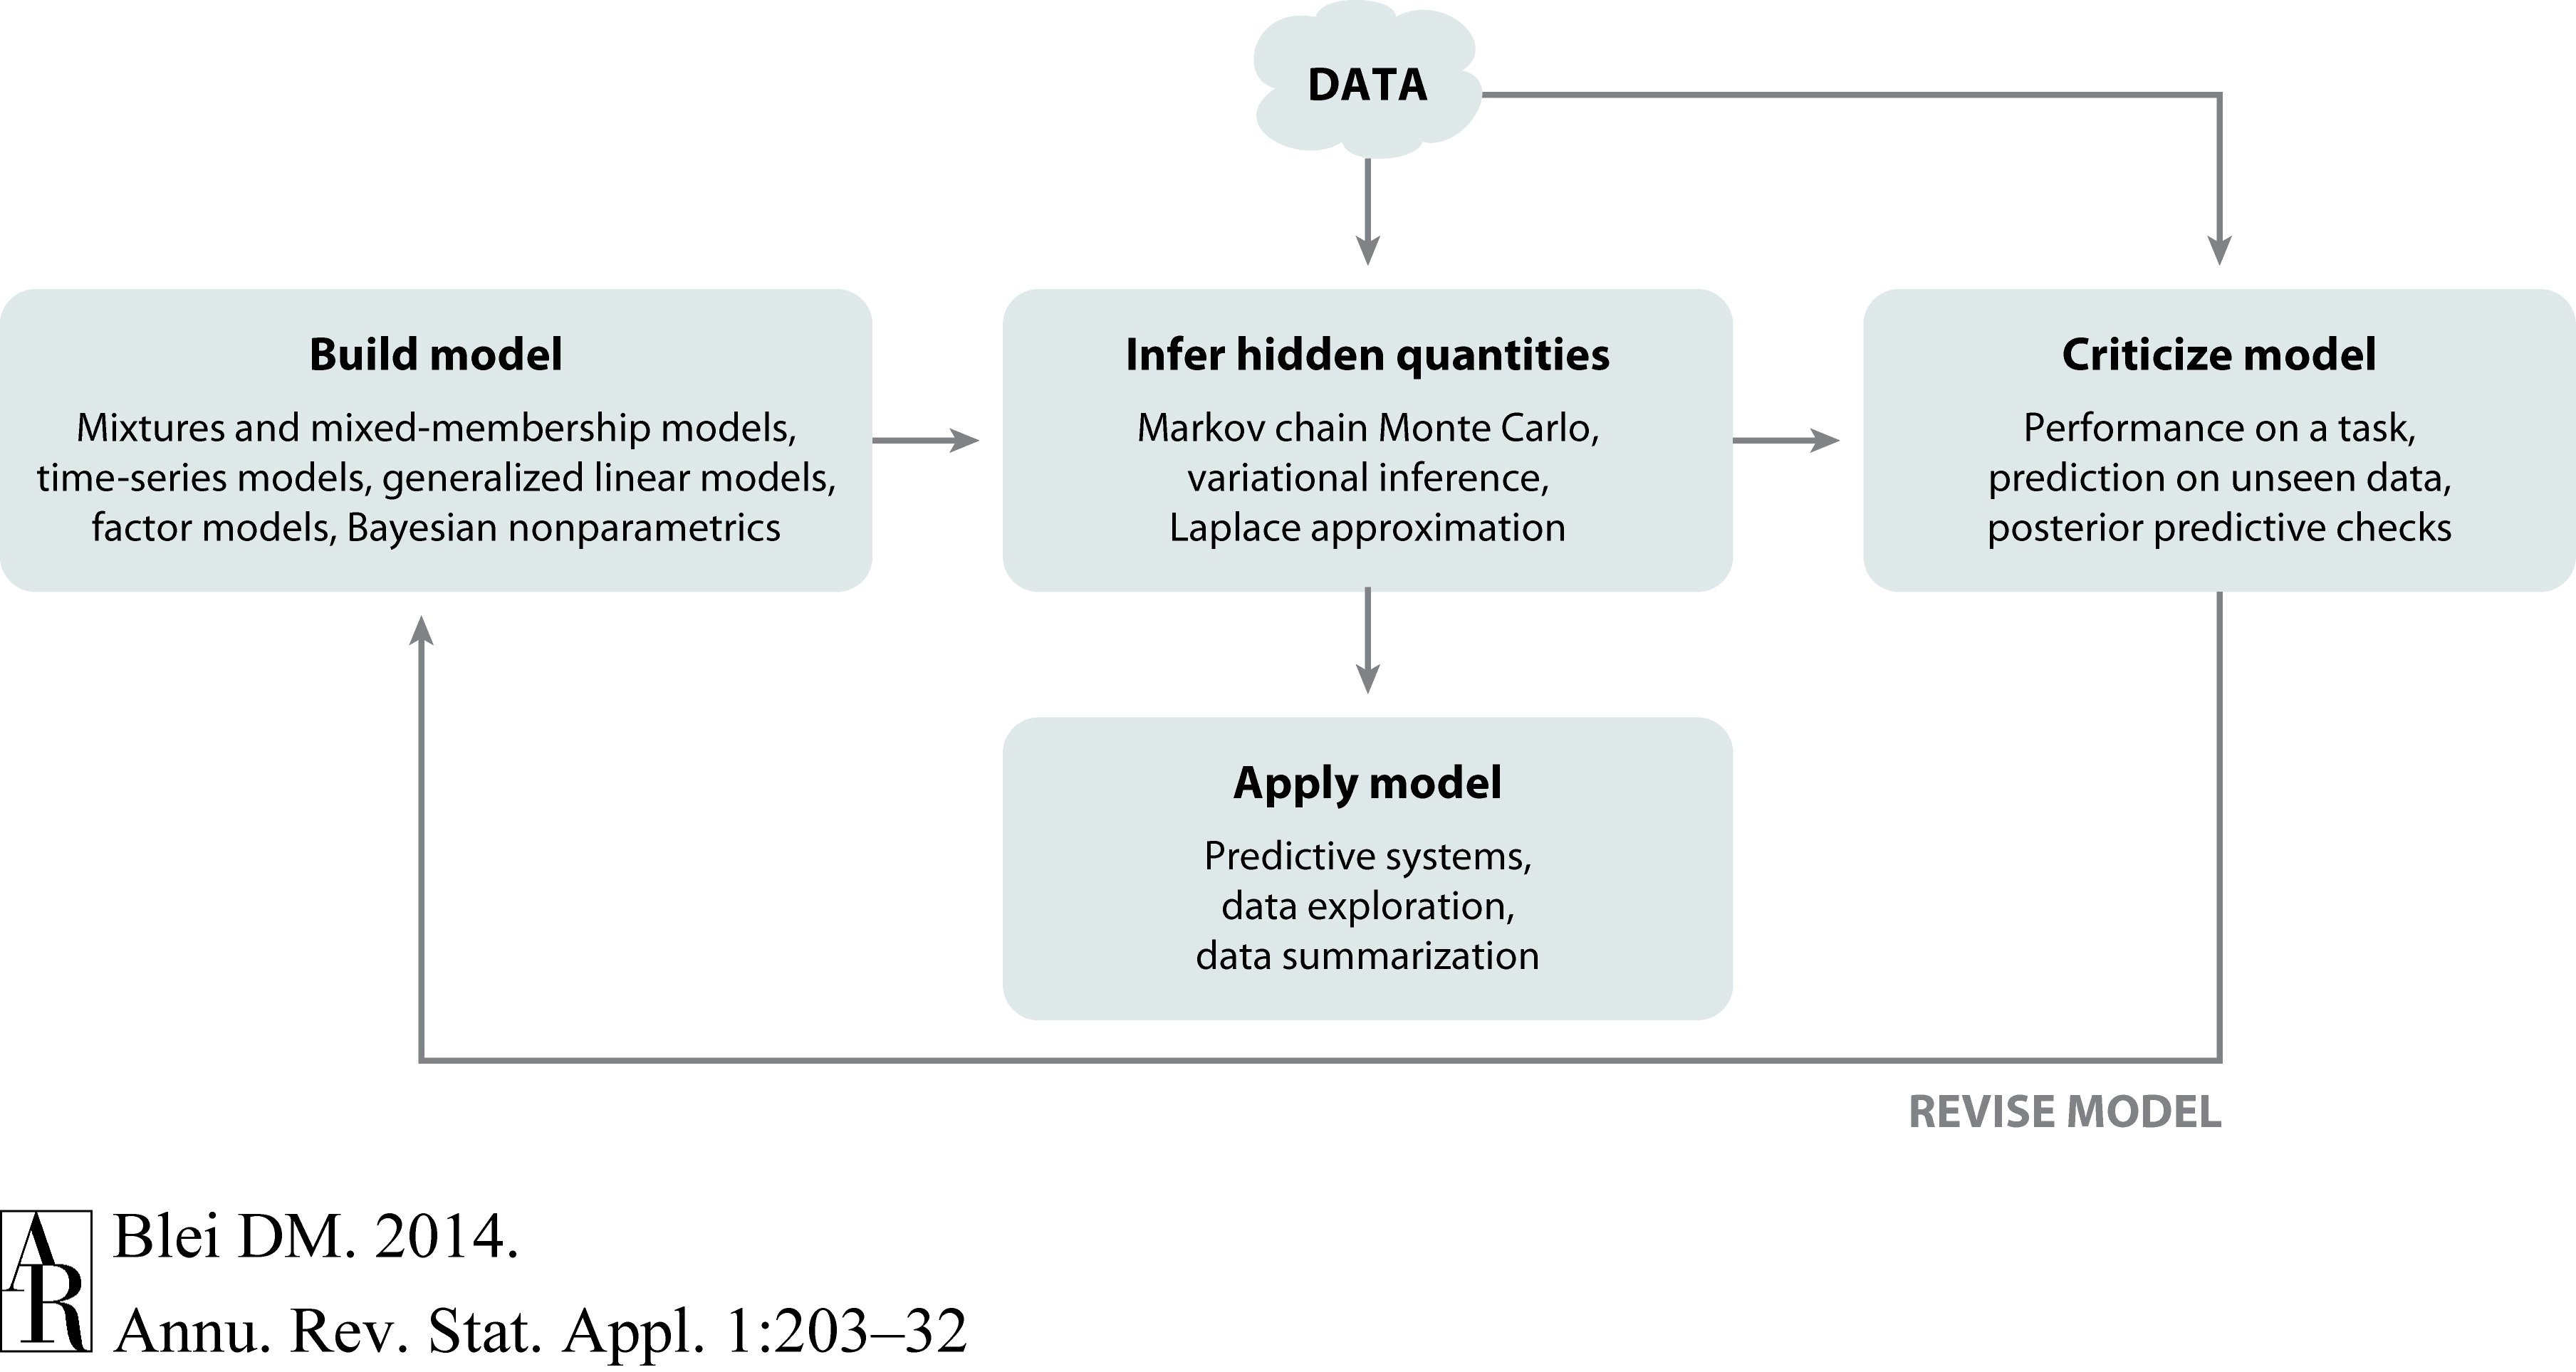
\includegraphics[width=.85\linewidth]{figures/lap1/boxsloop.jpeg}\\
\end{center} 
\begin{flushright}
{\footnotesize Blei, \textit{Ann. Rev. Stat. App.} 2014.}
\end{flushright}
\end{frame}

\begin{frame}{Lap 3: Robust regress models and Intro to MCMC}
\begin{itemize}
    \item \hyperref[sec:robust_regression]{\textbf{Model:} Robust regression models}
    \item \hyperref[sec:intro_mcmc]{\textbf{Algorithm:} Intro to Markov chain Monte Carlo (MCMC)}
    \item \hyperref[sec:diagnostics]{\textbf{Criticism:} MCMC Diagnostics}
    \item \hyperref[sec:hmc]{\textbf{Algorithm II:} Hamiltonian Monte Carlo}
\end{itemize}
\end{frame}


\section{Model: Robust regression models}
\label{sec:robust_regression}

\begin{frame}{Robustness to outliers}
\begin{columns}
\begin{column}{.5\textwidth}
Consider the following model:
\begin{align*}
    y_n &\sim \begin{cases}
    \cN(\mbw^\top \mbx_n, \sigma^2) & \text{with prob } 0.85 \\
    \cN(0, \sigma_{\mathsf{out}}^2) & \text{o.w.}
    \end{cases}
\end{align*}
where $\sigma_{\mathsf{out}}^2 \gg \sigma^2$.
\end{column}

\begin{column}{.5\textwidth}
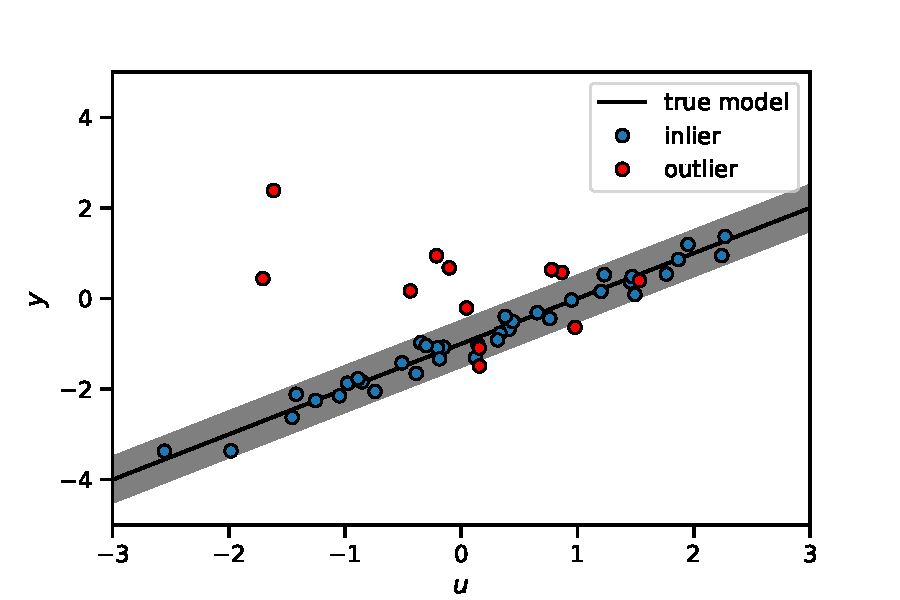
\includegraphics[width=\textwidth]{figures/lap3/data.pdf}
\end{column}

\end{columns}
\end{frame}

\begin{frame}{Robustness to outliers II}

A standard Bayesian linear regression (Lap 1) compensates by inferring different weights and a larger variance.

\centering
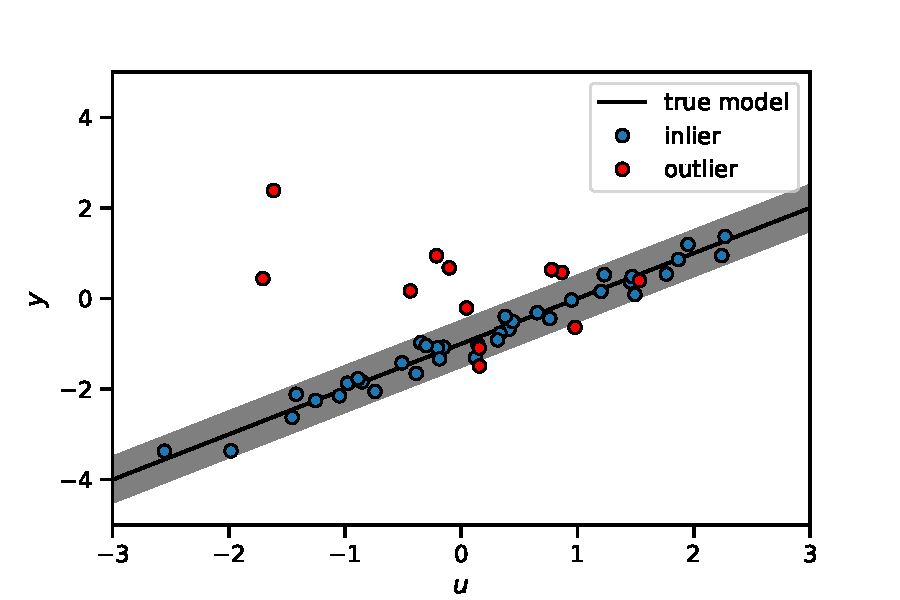
\includegraphics[width=.49\textwidth]{figures/lap3/data.pdf}
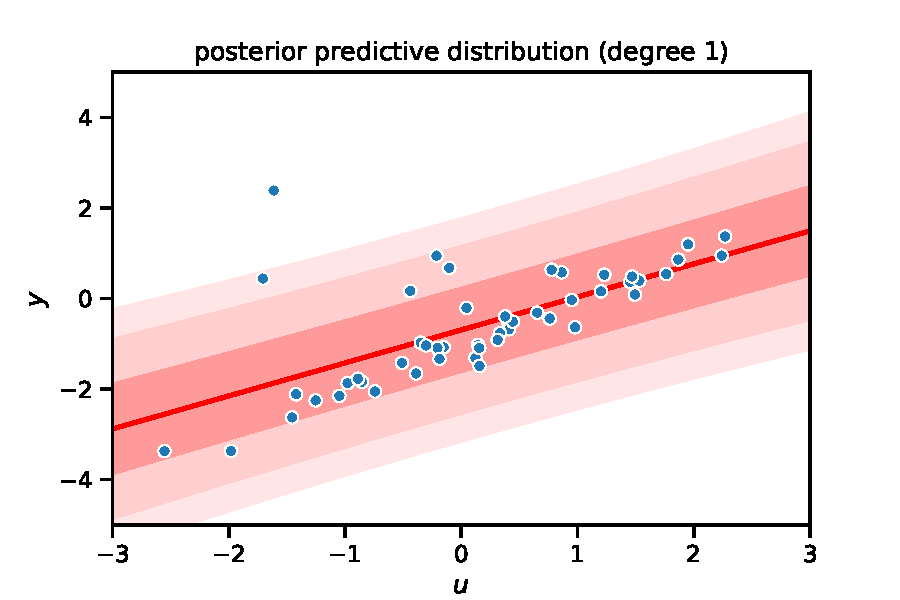
\includegraphics[width=.49\textwidth]{figures/lap3/post_pred.pdf}

\end{frame}

\begin{frame}{Robustness to outliers III}
We also see this in the posterior distribution of the weights...

\centering
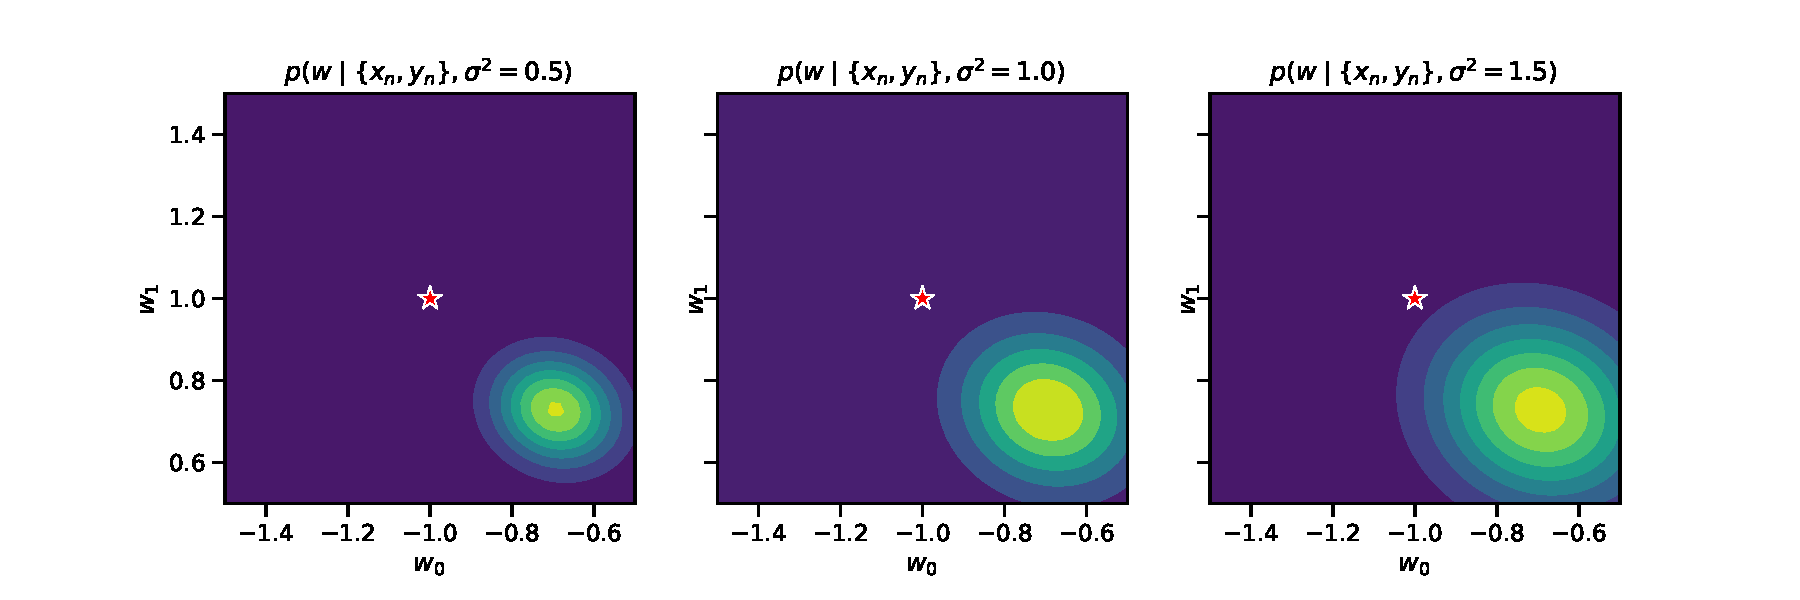
\includegraphics[width=.9\textwidth]{figures/lap3/w_post.pdf}
\end{frame}

\begin{frame}{Robustness to outliers IV}
...And in the posterior distribution of the variance

\centering
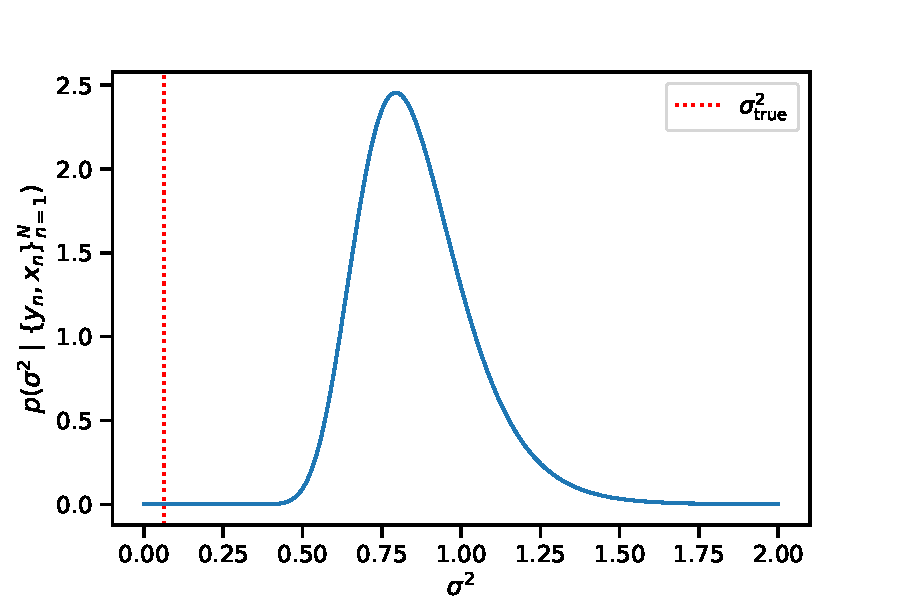
\includegraphics[width=.5\textwidth]{figures/lap3/sigmasq_post.pdf}
\end{frame}

\begin{frame}{Robust modeling with heavy tailed distributions}
One way to allow for outliers is via a discrete mixture distribution, like we used to simulate this data. More on this next week!

Mixtures are one way of creating \textit{heavy tailed} conditional distributions. I.e. they place more probability mass on observations far from the mean or mode.

Heavier tails allow the model to effectively downweight some observations when inferring the weights. In the discrete mixture example, if we knew which data points came from the outlier distribution, we would simply ignore them (set their weights to zero) when calculating the posterior distribution of the regression coefficients.

Of course, we don't \textit{a priori} which datapoints are inliers and which are outliers.  

Robust inference largely amounts to \textit{figuring out how to weight different observations} during inference.

\end{frame}

\begin{frame}{Student's t as a scale-mixture of Gaussians}
The Student's t distribution takes the discrete mixture idea to a continuous limit.

We can view the Student's distribution as a continuous \textit{scale-mixture of Gaussians},
\begin{align}
    t(y \mid \mu, \tau^2, \nu) &= \int \cN(y \mid \mu, \sigma^2) \, \distInvChiSq(\sigma^2 \mid \nu, \tau^2) \dif \sigma^2 \\
    &= \frac {\Gamma ({\frac {\nu +1}{2}})}{\Gamma ({\frac {\nu }{2}}){\sqrt {\pi \nu \tau^2}}} \left(1+{\frac {1}{\nu \tau^2}}\left(y-\mu \right)^{2}\right)^{-{\frac {\nu +1}{2}}}
\end{align}

Equivalently, we can think of $y \sim t(\mu, \tau^2, \nu)$ as arising from a two-step sampling procedure,
\begin{align}
    \sigma^2 &\sim \distInvChiSq(\nu, \tau^2) \\
    y &\sim \cN(\mu, \sigma^2).
\end{align}
First sample a random variance, then sample a Gaussian observation.

Look familiar? Recall the posterior predictive distribution in Bayesian linear regression.

\end{frame}

\begin{frame}{The Student's t distribution has heavy tails}

As the degree of freedom parameter $\nu$ goes to infinity, the Student's t converges to a Gaussian.

\centering
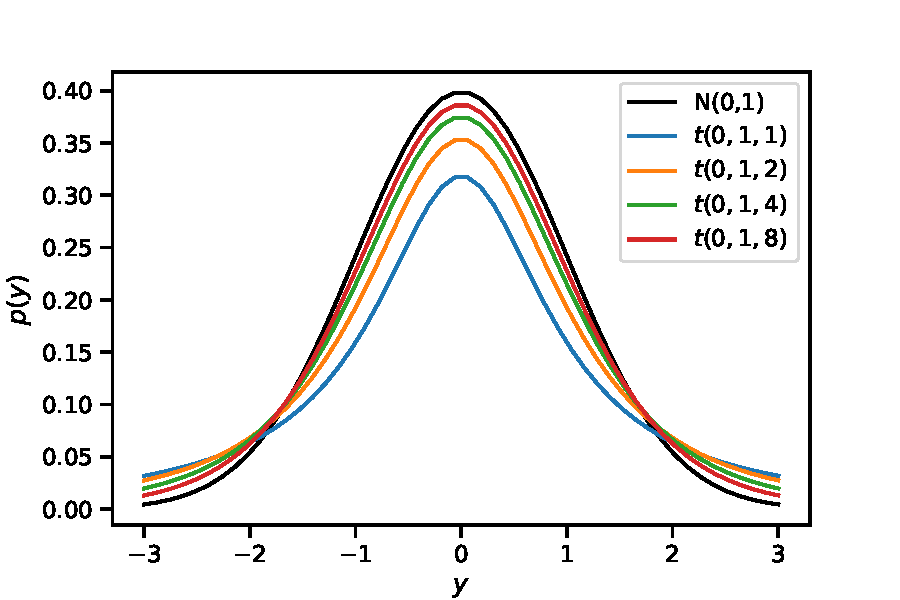
\includegraphics[width=.49\textwidth]{figures/lap3/t_pdf.pdf}
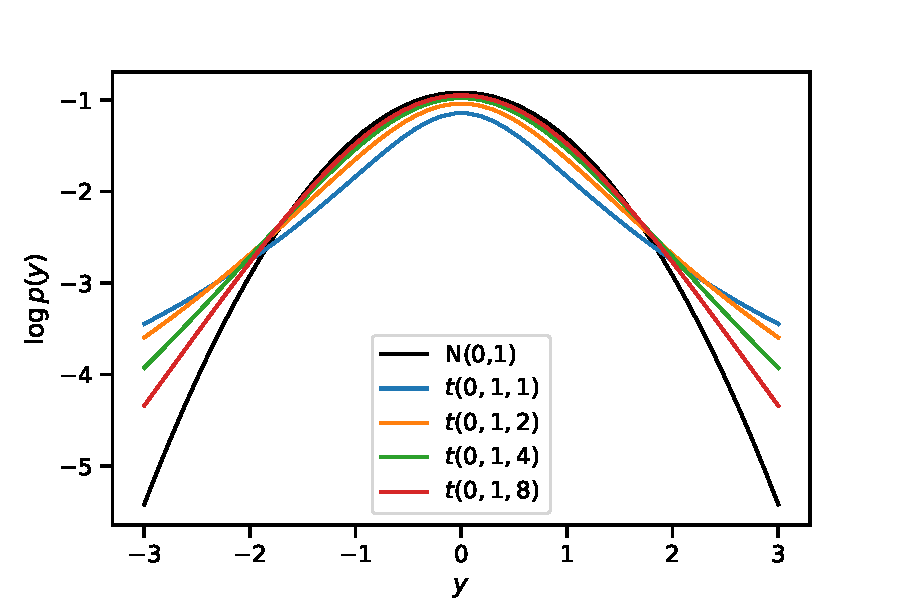
\includegraphics[width=.49\textwidth]{figures/lap3/t_logpdf.pdf}    

\end{frame}

\begin{frame}{Robust regression with Student's t noise model}

\textbf{Simple idea: } replace the normal distribution in Bayesian linear regression with a Student's t.

\begin{align}
    y_n \sim t(\mbw^\top \mbx_n, \tau^2, \nu) \iff 
    \sigma_n^2 &\sim \distInvChiSq(\nu, \tau^2)  \\
    y_n &\sim \cN(\mbw^\top \mbx_n, \sigma_n^2).
\end{align}

We can think of this as giving each datapoint its own random variance $\sigma_n^2$.

How does this relate to ``reweighting'' various datapoints? Suppose we somehow knew the variances $\sigma_n^2$ and just needed to infer the parameters $\mbw$. Recall that sufficient statistics for $\mbw$ where $\sum_{n=1}^N \frac{y_n \mbx_n}{\sigma_n^2}$, $\sum_{n=1}^N \frac{\mbx_n \mbx_n^\top }{\sigma_n^2}$, and $\sum_{n=1}^N \frac{1}{\sigma_n^2}$. Effectively, datapoints with larger variance contribute less to the sufficient statistics.

\end{frame}

\begin{frame}{Probabilistic model}

Unfortunately, we don't know the variances (knowing the variances is like knowing which datapoints are outliers) so we have to work with the $t$ distribution instead.

Our likelihood is,
\begin{align}
    p(\{y_n\}_{n=1}^N \mid \mbw, \tau^2, \nu, \{\mbx_n\}_{n=1}^N) 
    &= \prod_{n=1}^N t(y_n \mid \mbw^\top \mbx_n, \tau^2, \nu) \\
    &= \prod_{n=1}^N \frac {\Gamma ({\frac {\nu +1}{2}})}{\Gamma ({\frac {\nu }{2}}){\sqrt {\pi \nu \tau^2}}} \left(1+{\frac {1}{\nu \tau^2}}\left(y_n-\mbw^\top \mbx_n \right)^{2}\right)^{-{\frac {\nu +1}{2}}}
\end{align}
This doesn't simplify, but it is differentiable and easy to compute any point $(\mbw, \tau^2, \nu)$.

To complete the model, assume a broad Gaussian prior on the \emph{log} of non-negative parameters,
\begin{align}
    p(\log \tau^2, \log \nu) &= \cN(\log \tau^2 \mid 0, 3) \, \cN(\log \nu \mid 0, 3),
\end{align}
and an improper uniform prior on the weights.

A Gaussian prior on the log of a parameter is equivalent to a \textit{log normal} prior on the parameter.

\end{frame}

\begin{frame}{Visualizing the log joint probability}
\centering
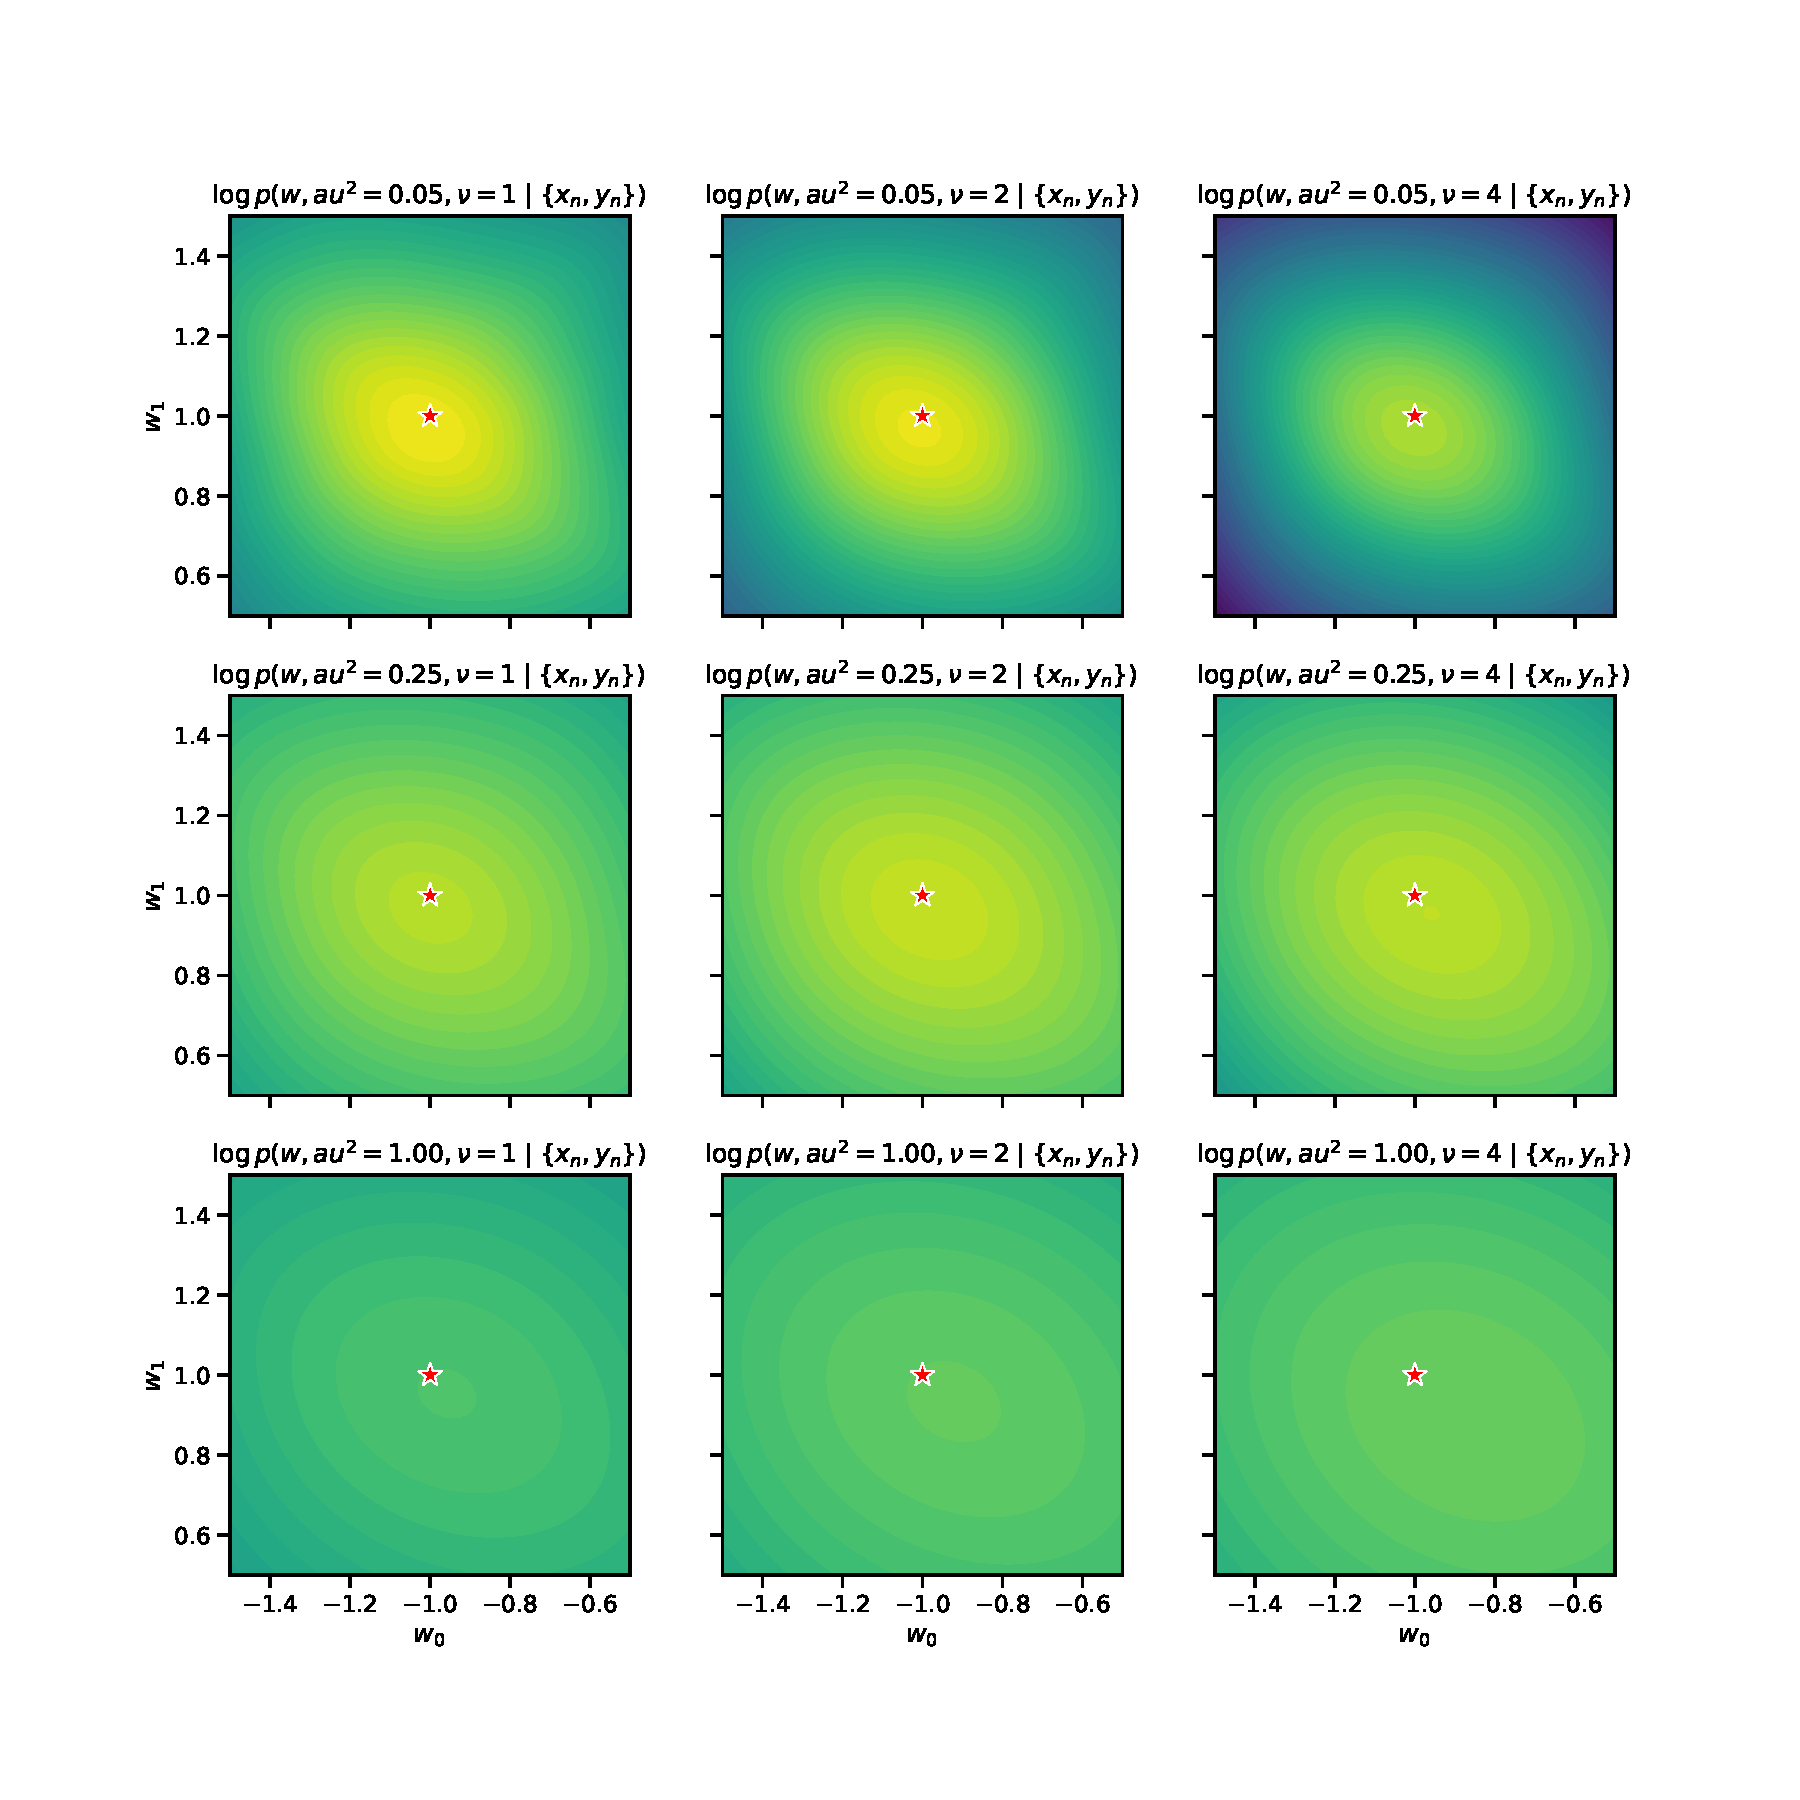
\includegraphics[width=.6\textwidth]{figures/lap3/robust_w_post.pdf}
\end{frame}

\begin{frame}{Visualizing the log joint probability II}
\centering
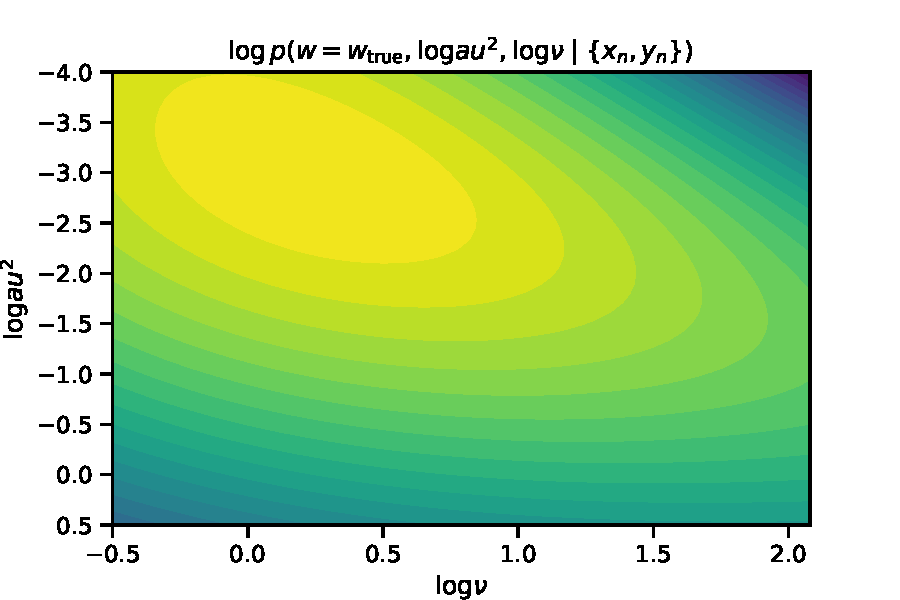
\includegraphics[width=.7\textwidth]{figures/lap3/robust_post.pdf}
\end{frame}

\begin{frame}{MAP Estimation}

Again, the posterior doesn't have a simple analytical form, but we can still try our tools from last week. E.g. we can use black box optimizers to find the mode.

\centering
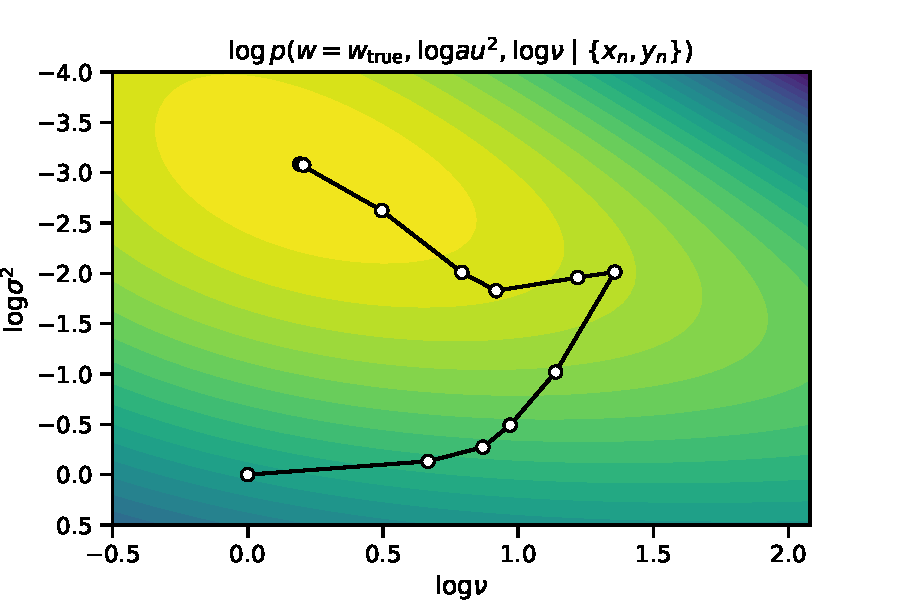
\includegraphics[width=.7\textwidth]{figures/lap3/robust_post2.pdf}
    
\end{frame}

\begin{frame}{Predictive distribution with $\mbw_{\mathsf{MAP}}$}

The MAP estimate of the parameters yields a much better estimate of the weights by allowing for a heavy tailed distribution of outliers.

\centering
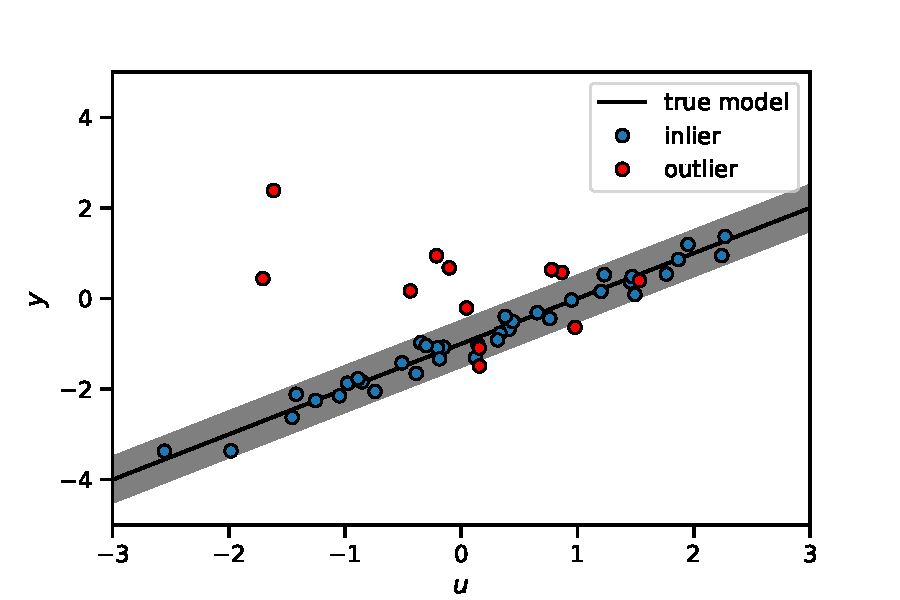
\includegraphics[width=.49\textwidth]{figures/lap3/data.pdf}
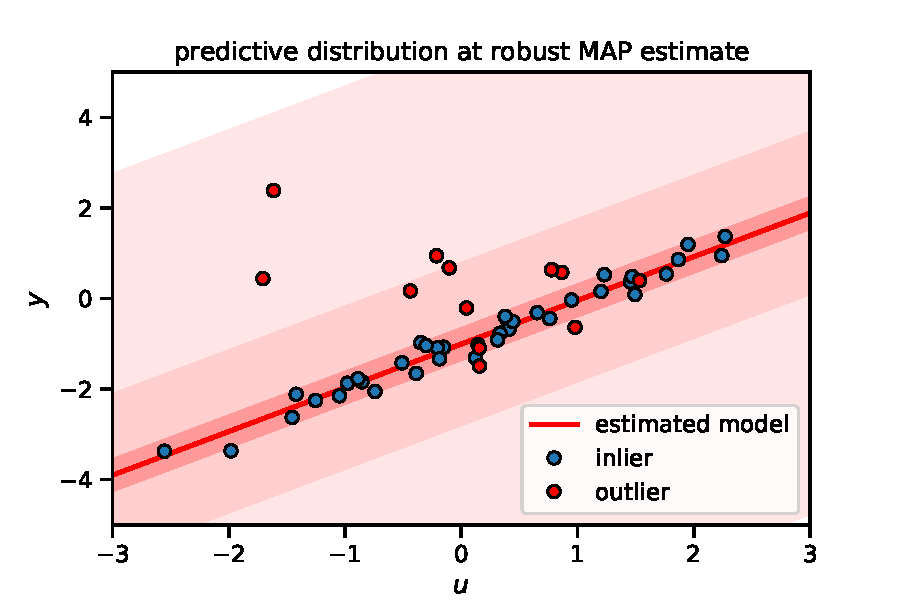
\includegraphics[width=.49\textwidth]{figures/lap3/robust_map_pred.pdf}
    
\end{frame}

\section{Algorithm: Intro to MCMC}
\label{sec:intro_mcmc}

\begin{frame}{Lap 3: Robust regress models and Intro to MCMC}
\begin{itemize}
    \item \hyperref[sec:robust_regression]{Model: Robust regression models}
    \item \hyperref[sec:intro_mcmc]{\textbf{Algorithm: Intro to Markov chain Monte Carlo (MCMC)}}
    \item \hyperref[sec:diagnostics]{Criticism: MCMC Diagnostics}
    \item \hyperref[sec:hmc]{Algorithm II: Hamiltonian Monte Carlo}
\end{itemize}
\end{frame}


\begin{frame}{Notation}
\begin{itemize}
    \item Let $\mbtheta \in \Theta$ denote the model parameters. 
    \begin{itemize}
        \item In robust regression, $\mbtheta = (\mbw, \tau^2, \nu) \in \reals^P \times \reals_+ \times \reals_+$.
    \end{itemize}
    
    \item Let $\cD = \{\mbx_n, y_n\}_{n=1}^N$ denote the observed data.
\end{itemize}
    
\end{frame}

\begin{frame}{Posterior expectations}
% Approximate expectations under the posterior via samples
The central object of Bayesian inference is the posterior distribution, $p(\mbtheta \mid \cD)$.

However, we almost always interact with the posterior distribution through \emph{expectations}.

\begin{itemize}
    \item $\E_{p(\mbtheta | \cD)}[\mbtheta]$, the posterior mean.
    \item $\E_{p(\mbtheta | \cD)}[\bbI[\mbtheta \in \cA]]$, the probability of the parameters being in set $\cA$.
    \item $\E_{p(\mbtheta | \cD)}[p(\cD' \mid \mbtheta)]$, the posterior predictive density of new data $\cD'$.
\end{itemize}

All of these can be written as $\E_{p(\mbtheta | \cD)}[f(\mbtheta)]$ for some function $f$.

(One exception is the posterior mode, which is not so easily expressed as an expectation.)
\end{frame}

\begin{frame}{Approximating posterior expectations}
Generally, we can't analytically compute posterior expectations. (\emph{Why not?})
    
In these cases, we need to resort to approximations.

For example, we could use \emph{quadrature methods} like Simpon's rule or the trapezoid rule to numerically approximate the integral over $\Theta$. 

Roughly,
\begin{align}
    \E_{p(\mbtheta | \cD)}[f(\mbtheta)] &\approx \sum_{m=}^M p(\mbtheta_m \mid \cD) \, f(\mbtheta_m) \, \Delta_m
\end{align}
where $\mbtheta_m \subset \Theta$ is a grid of points and $\Delta_m$ is a volume around that point.

This works for low dimensional problems (say, up to $5$ dimensions), but the number of points ($M$) needed to get a good estimate grows exponentially with the parameter dimension.

\end{frame}

\begin{frame}{Monte Carlo approximations}

\textbf{Idea:} approximate the expectation via sampling,

\begin{align}
    \E_{p(\mbtheta | \cD)}[f(\mbtheta)] &\approx \frac{1}{S} \sum_{s=1}^S f(\mbtheta_s) 
    \quad \text{where} \quad
    \mbtheta_s \sim p(\mbtheta \mid \cD).
\end{align}

Let $\hat{f} = \frac{1}{S} \sum_{s=1}^S f(\mbtheta_s)$ denote the Monte Carlo estimate. It is a random variable, since it's a function of random samples $\mbtheta_s$. 

As such we can reason about its mean and variance. Clearly,
\begin{align}
    \E[\hat{f}] = \frac{1}{S} \sum_{s=1}^S \E_{p(\mbtheta | \cD)}[f(\mbtheta)] = \E_{p(\mbtheta | \cD)}[f(\mbtheta)].
\end{align}
Thus, $\hat{f}$ is an \emph{unbiased} estimate of the desired expectation.

\end{frame}

\begin{frame}{Monte Carlo approximations II}

What about its variance?
\begin{align}
    \Var[\hat{f}] 
    &= \Var \left(\frac{1}{S} \sum_{s=1}^S f(\mbtheta_s) \right) \\
    &= \frac{1}{S^2} \left( \sum_{s=1}^S \Var[f(\mbtheta)] + 2 \sum_{1 \leq s < s' \leq S} \mathrm{Cov} [f(\mbtheta_s),  f(\mbtheta_{s'})] \right)
\end{align}

If the samples are not only identically distributed but also \emph{uncorrelated}, then~$\Var[\hat{f}] = \frac{1}{S} \Var[f(\mbtheta)]$.

In this case, the \emph{root mean squared error} (RMSE) of the estimate is $\sqrt{\Var[\hat{f}]} = O(S^{-\frac{1}{2}})$.

Compare this to Simpson's rule, which for smooth 1D problems has error rate~$O(S^{-4})$. That's roughly 8 times better!

However, for multidimensional problems, Simpson's rule is $O(S^{-\frac{4}{P}})$, whereas the \textbf{error rate of Monte Carlo does not depend on the dimensionality!}

\end{frame}

\begin{frame}{The Catch}

So far so good: we'll just draw a lot of samples to drive down our Monte Carlo error. 

\textbf{Here's the catch!} How do you draw samples from the posterior $p(\mbtheta \mid \cD)$?

We're interested in Monte Carlo for cases where the posterior does not admit a simple closed form!

In general, sampling the posterior is as hard as computing the marginal likelihood. 

\end{frame}

\begin{frame}{Markov chain Monte Carlo (MCMC)}

\textbf{Idea:} Design a Markov chain whose stationary distribution is the posterior.
    
\centering
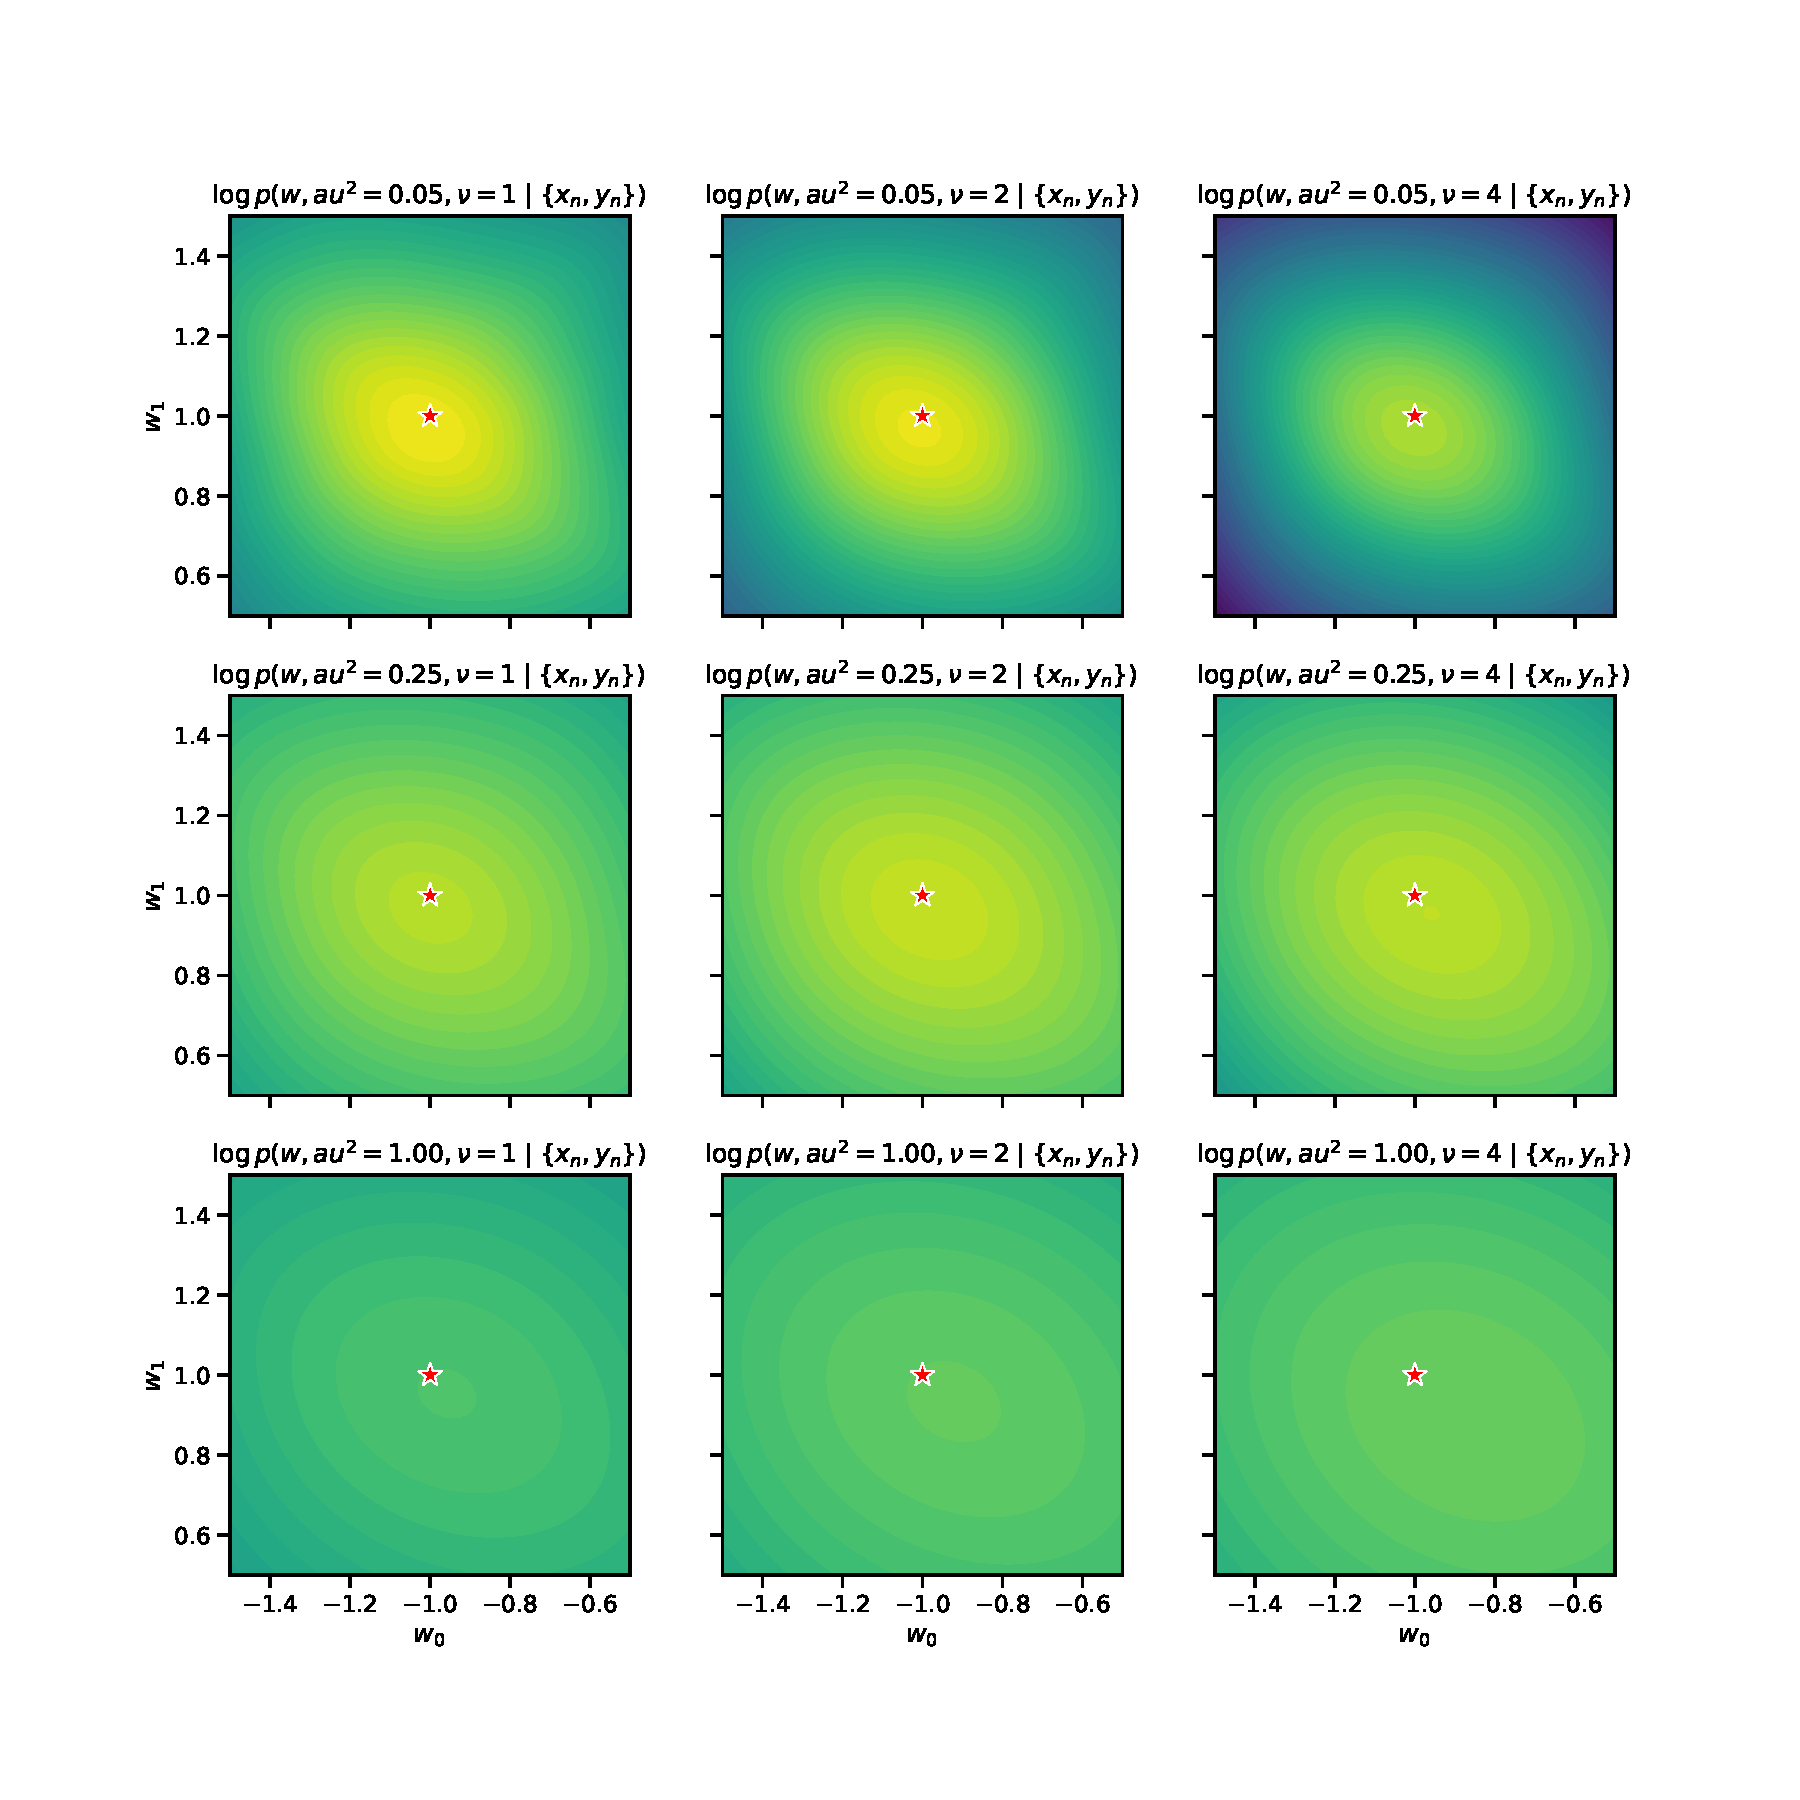
\includegraphics[width=.5\textwidth]{figures/lap3/robust_w_post.pdf}

\end{frame}

\begin{frame}{Markov chains}
    
A \emph{Markov chain} is a joint distribution of a sequence of variables, $\pi(\mbtheta_1, \mbtheta_2, \ldots, \mbtheta_S)$.

(To avoid confusion with the model $p$, we denote the densities associated with the Markov chain by $\pi$.)

The Markov chain factorizes so that each variable is drawn conditional on the previous variable,
\begin{align}
    \pi(\mbtheta_1, \mbtheta_2, \ldots, \mbtheta_S)
    &= 
    \pi_{1}(\mbtheta_1) \prod_{s=2}^S \pi(\mbtheta_s \mid \mbtheta_{s-1}).
\end{align}
This is called the \emph{Markov property}.

The distribution $\pi_1(\mbtheta_1)$ is called the \textit{initial distribution}.

The distribution $\pi(\mbtheta_s \mid \mbtheta_{s-1})$ is called the \textit{transition distribution}. If the transition distribution is the same for each $s$, the Markov chain is \textit{homogenous}.
\end{frame}

\begin{frame}{Stationary distributions}
Let $\pi_s(\mbtheta_s)$ denote the marginal distribution of sample $\mbtheta_s$. It can be obtained recursively as,
\begin{align}
    \pi_s(\mbtheta_s) &= \int \pi_{s-1}(\mbtheta_{s-1}) \, \pi(\mbtheta_s \mid \mbtheta_{s-1}) \dif \mbtheta_{s-1}.
\end{align}
We are interested in the asymptotic behavior of the marginal distributions as $s \to \infty$.

A distribution $\pi^*(\mbtheta)$ is a \textbf{stationary distribution} if,
\begin{align}
    \pi^*(\mbtheta) &= \int \pi^*(\mbtheta') \, \pi(\mbtheta \mid \mbtheta') \dif \mbtheta'.
\end{align}
That is, suppose the marginal of sample $\mbtheta'$ is $\pi^*(\mbtheta)$. Then the marginal of the next time point is also~$\pi^*(\mbtheta)$.
\end{frame}

\begin{frame}{Detailed balance}
    
% \textbf{Our goal} is to design a Markov chain where \textit{the posterior distribution is the unique stationary distribution}. That is, we want~$\pi^*(\mbtheta) = p(\mbtheta \mid \cD)$.

How can we relate transition distributions and stationary distributions?

A sufficient (but not necessary) condition for $\pi^*(\mbtheta)$ to be a stationary distribution is that it satisfies \textit{detailed balance},
\begin{align}
    \pi^*(\mbtheta') \pi(\mbtheta \mid \mbtheta') &=
    \pi^*(\mbtheta) \pi(\mbtheta' \mid \mbtheta) 
\end{align}
In words, the probability of starting at $\mbtheta'$ and moving to $\mbtheta$ is the same as that of starting at $\mbtheta$ and moving to $\mbtheta'$, if you draw the starting point from the stationary distribution.

To see that detailed balance is sufficient, integrate both sides to get,
\begin{align}
    \int \pi^*(\mbtheta') \pi(\mbtheta \mid \mbtheta') \dif \mbtheta'
    &=
    \int \pi^*(\mbtheta) \pi(\mbtheta' \mid \mbtheta) \dif \mbtheta'
    =
    \pi^*(\mbtheta) \int \pi(\mbtheta' \mid \mbtheta) \dif \mbtheta'
    = \pi^*(\mbtheta).
\end{align}
Thus, $\pi^*(\mbtheta)$ is a stationary distribution of the Markov chain with transitions $\pi(\theta \mid \theta')$.

\end{frame}

\begin{frame}{Ergodicity}
Detailed balance can be used to show that $\pi^*(\mbtheta)$ is \textit{a} stationary distribution, but not that it is \textit{the unique} one.

This is where \textit{ergodicity} comes in. A Markov chain is ergodic if $\pi_s(\mbtheta_s) \to \pi^\star(\mbtheta)$ regardless of $\pi_1(\mbtheta_1)$.

An ergodic chain has only one stationary distribution, $\pi^*(\mbtheta)$. 

The easiest way to prove ergodicity is to show that it is possible to reach any $\mbtheta'$ from any other $\mbtheta$. E.g. this is trivially so if $\pi(\mbtheta' \mid \mbtheta) > 0$. 

Note: a more technical definition is that all pairs of sets \textit{communicate}, in which case the chain is \textit{irreducible}, and that each state is \textit{aperiodic}. The definitions can be a bit overwhelming.

\end{frame} 

\begin{frame}{The Metropolis-Hastings algorithm}

Finally we come to our \textbf{main objective}: designing a Markov chain for which \textit{the posterior is the unique stationary distribution.} 

That is, we want $\pi^*(\mbtheta) = p(\mbtheta \mid \cD)$.

Recall our \textbf{constraint}: we can only compute the joint probability (the numerator in Bayes' rule), not the marginal likelihood (the denominator).

Fortunately, that still allows us to compute ratios of posterior densities! We have,
\begin{align}
    \frac{p(\mbtheta \mid \cD)}{p(\mbtheta' \mid \cD)} 
    &= 
    \frac{p(\mbtheta, \cD)}{p(\cD)} \frac{p(\cD)}{p(\mbtheta',  \cD)} 
    = \frac{p(\mbtheta, \cD)}{p(\mbtheta',  \cD)}.
\end{align}
    
\end{frame}

\begin{frame}{The Metropolis-Hastings algorithm II}
    
Now rearrange the detailed balance condition to relate ratios of transition probabilities to ratios of joint probabilities,
\begin{align}
    \label{eq:transition_constraint}
    \frac{\pi(\mbtheta \mid \mbtheta')}{\pi(\mbtheta' \mid \mbtheta)}
    &= 
    \frac{\pi^*(\mbtheta)}{\pi^*(\mbtheta')}
    = 
    \frac{p(\mbtheta \mid \cD)}{p(\mbtheta' \mid \cD)}
    = 
    \frac{p(\mbtheta, \cD)}{p(\mbtheta',  \cD)}
\end{align}

To construct such a transition distribution $\pi(\mbtheta \mid \mbtheta')$, break it down into two steps. 
\begin{enumerate}
    \item Sample a proposal $\mbtheta$ from a \emph{proposal distribution} $q(\mbtheta \mid \mbtheta')$,
    \item Accept the proposal with \emph{acceptance probability}~$a(\mbtheta' \to \mbtheta)$. (Otherwise, set $\mbtheta = \mbtheta'$.)
\end{enumerate}

Thus,
\begin{align}
    \pi(\mbtheta \mid \mbtheta') &= 
    \begin{cases}
    q(\mbtheta \mid \mbtheta') \, a(\mbtheta' \to \mbtheta) & \text{if } \mbtheta' \neq \mbtheta \\
    \int q(\mbtheta'' \mid \mbtheta') \, (1 - a(\mbtheta' \to \mbtheta'')) \dif \mbtheta'' & \text{if } \mbtheta' = \mbtheta
    \end{cases}
\end{align}

\end{frame}

\begin{frame}{The Metropolis-Hastings algorithm III}
The constraint in \eqref{eq:transition_constraint} is trivially satisfied when $\mbtheta = \mbtheta'$. When $\mbtheta \neq \mbtheta'$, we need
\begin{multline}
    \frac{\pi(\mbtheta \mid \mbtheta')}{\pi(\mbtheta' \mid \mbtheta)}
    = 
    \frac{q(\mbtheta \mid \mbtheta') \, a(\mbtheta' \to \mbtheta)}{q(\mbtheta' \mid \mbtheta) \, a(\mbtheta \to \mbtheta')}
    = 
    \frac{p(\mbtheta, \cD)}{p(\mbtheta',  \cD)}
    \Rightarrow
    \frac{a(\mbtheta' \to \mbtheta)}{a(\mbtheta \to \mbtheta')}
    = 
    \underbrace{\frac{p(\mbtheta, \cD) \, q(\mbtheta' \mid \mbtheta)}{p(\mbtheta',  \cD) \, q(\mbtheta \mid \mbtheta') }}_{\triangleq A(\mbtheta' \to \mbtheta)}
\end{multline}

WLOG, assume $ A(\mbtheta' \to \mbtheta) \leq 1$. (If it's not, its inverse $A(\mbtheta \to \mbtheta')$ must be.) 

A simple way to ensure detailed balance is to set $a(\mbtheta' \to \mbtheta) = A(\mbtheta' \to \mbtheta)$ and $a(\mbtheta \to \mbtheta') = 1$. 

We can succinctly capture both cases with,
\begin{align}
    a(\mbtheta' \to \mbtheta) &= 
    \min \left\{1, \, A(\mbtheta' \to \mbtheta) \right \} = 
    \min \left\{1, \, \frac{p(\mbtheta, \cD) \, q(\mbtheta' \mid \mbtheta)}{p(\mbtheta',  \cD) \, q(\mbtheta \mid \mbtheta')} \right \}.
\end{align}

\end{frame} 

\begin{frame}{The Metropolis algorithm}
    Now consider the special case in which the proposal distribution is symmetric; i.e. $q(\mbtheta \mid \mbtheta') = q(\mbtheta' \mid \mbtheta)$.
    
    Then the proposal densities cancel in the acceptance probability and,
    \begin{align}
    a(\mbtheta' \to \mbtheta) &= 
        \min \left\{1, \, \frac{p(\mbtheta, \cD)}{p(\mbtheta',  \cD)} \right \}.
    \end{align}

    In other words, you accept any proposal that moves ``uphill,'' and only accept ``downhill'' moves with some probability. 
    
    This is called the \textit{Metropolis algorithm} and it has close connections to \textit{simulated annealing}.
\end{frame}

% MH example, trace plots
\begin{frame}{Metropolis-Hastings Trace Plot}

Proposal distribution: $q(\mbtheta \mid \mbtheta') = \cN(\mbtheta \mid \mbtheta', 0.1 \mbI)$; Initial distribution: $\pi_1(\mbtheta) = \delta_{\mbzero}(\mbtheta)$. Red lines show the MAP estimate; black lines show samples.
    
    \begin{center}
    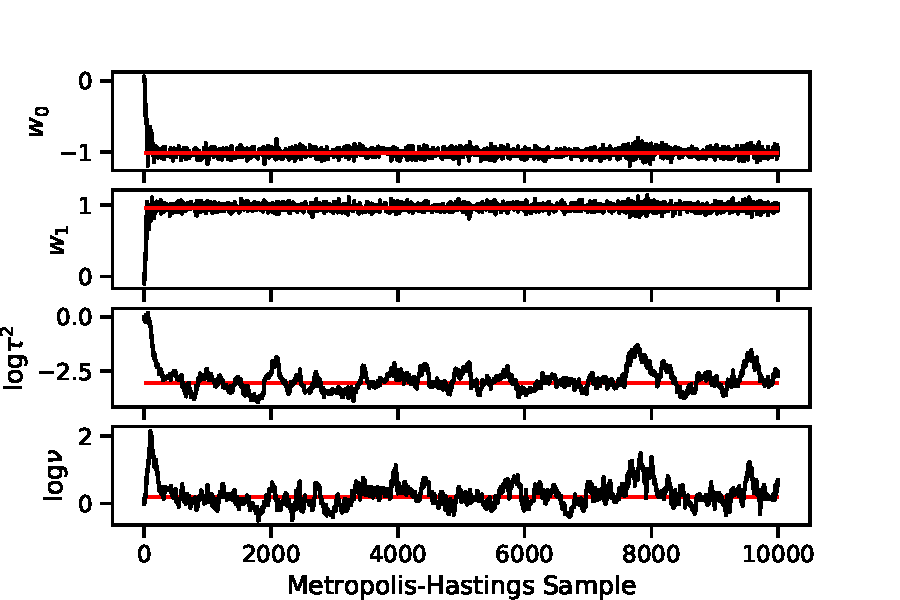
\includegraphics[width=0.6\textwidth]{figures/lap3/mh_traces.pdf}
    \end{center}
    
\end{frame}

\begin{frame}{Metropolis-Hastings Density Approximation}
    \centering
    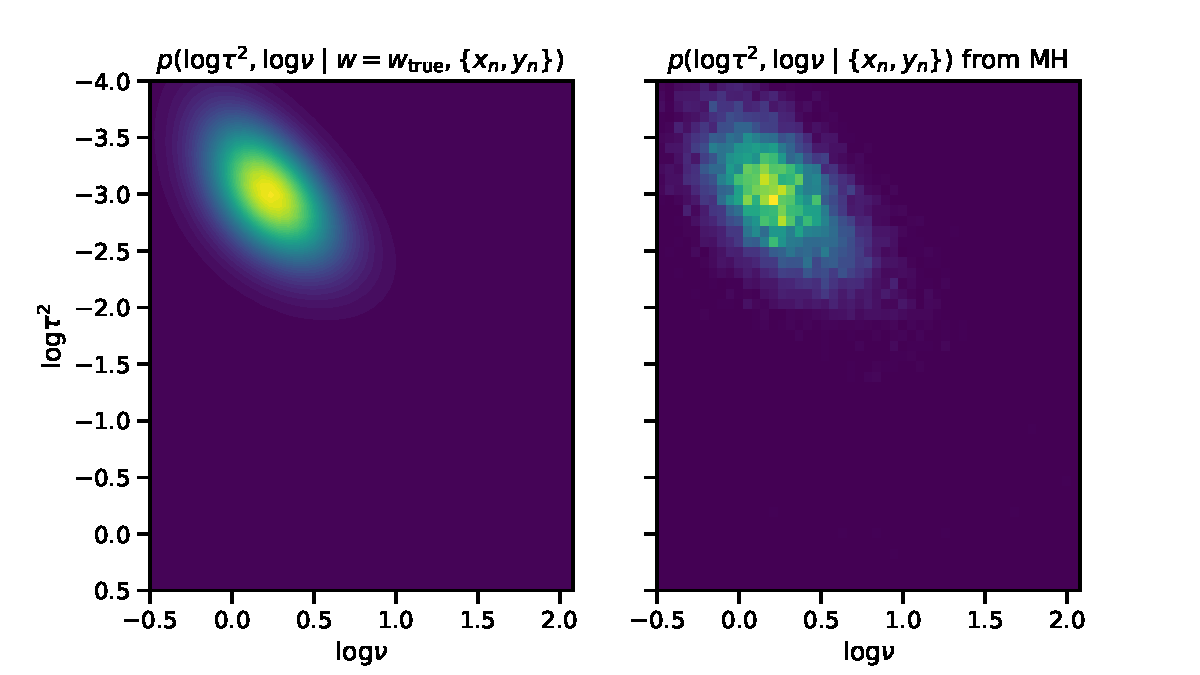
\includegraphics[width=0.6\textwidth]{figures/lap3/mh_nu_tausq_density.pdf}
\end{frame}

\section{MCMC Diagnostics}
\label{sec:diagnostics}

\begin{frame}{Lap 3: Robust regress models and Intro to MCMC}
\begin{itemize}
    \item \hyperref[sec:robust_regression]{Model: Robust regression models}
    \item \hyperref[sec:intro_mcmc]{Algorithm: Intro to Markov chain Monte Carlo (MCMC)}
    \item \hyperref[sec:diagnostics]{\textbf{Criticism: MCMC Diagnostics}}
    \item \hyperref[sec:hmc]{Algorithm II: Hamiltonian Monte Carlo}
\end{itemize}
\end{frame}

\begin{frame}{Autocovariance and autocorrelation}
Recall that,
\begin{align}
    \Var[\hat{f}] 
    &= \frac{1}{S^2} \left( \sum_{s=1}^S \Var[f(\mbtheta)] + 2 \sum_{1 \leq s < s' \leq S} \mathrm{Cov} [f(\mbtheta_s),  f(\mbtheta_{s'})] \right) \\
    &\approx \frac{1}{S} \left(\Var[f(\mbtheta)] + 2\sum_{\ell=1}^{S} \mathrm{Cov} [f(\mbtheta_s),  f(\mbtheta_{s+\ell})] \right)
\end{align}
since the covariance is only a function of the lag $\ell$ once the chain has reached stationarity.

\textbf{Note:} At stationarity, the samples are identically distributed but still correlated!

$\mathrm{Cov} [f(\mbtheta_s),  f(\mbtheta_{s+\ell})] $ is called the \textit{autocovariance}. It's a function of the lag $\ell$ (and the function $f$).

The \textit{autocorrelation function} (ACF) is defined as, $\mathrm{acf}_f(\ell) = \mathrm{Cov} [f(\mbtheta_s),  f(\mbtheta_{s+\ell})] / \Var[f(\theta)]$ so
\begin{align}
    \Var[\hat{f}] 
    &\approx S^{-1} \, \Var[f(\mbtheta)] \left(1 + 2\sum_{\ell=1}^{S} \mathrm{acf}_f[\ell] \right).
\end{align}

\end{frame}


\begin{frame}{Effective sample size}
The \textit{effective sample size} (ESS) approximates the effective number of independent samples you get from an autocorrelated chain, in terms of the variance of the Monte Carlo estimate,
\begin{align}
    S_{\mathsf{eff},f} &= S \frac{\Var[f(\theta)]}{\Var[f(\theta)] ( 1 + 2 \sum_{\ell=1}^\infty \mathrm{acf}_f[\ell]) }
    =  \frac{S}{1 + 2 \sum_{\ell=1}^\infty \mathrm{acf}_f[\ell] }
\end{align}
and we let $S_{\mathsf{eff}}$ denote the ESS of the identity functional $f(\theta)= \theta$.

You have to be a bit careful when estimating the ESS---for large values of $\ell$ the sample correlation is too noisy. Typically, we stop when the sample acf is negative. See Section 11.5 of BDA3 for more details.

In practice, there are already good implementations in Python (c.f. \href{https://www.tensorflow.org/probability/api_docs/python/tfp/mcmc/effective_sample_size}{\texttt{tfp.stats.effective\_sample\_size}}) and R (c.f. the \href{https://cran.r-project.org/web/packages/coda/index.html}{\texttt{coda}} package). 
\end{frame}


\begin{frame}{Autocorrelation of the MH trace above}
    We used \href{https://www.tensorflow.org/probability/api_docs/python/tfp/stats/auto_correlation}{\texttt{tfp.stats.auto\_correlation}} to compute the autocorrelation function for the traces above,
    \begin{center}
         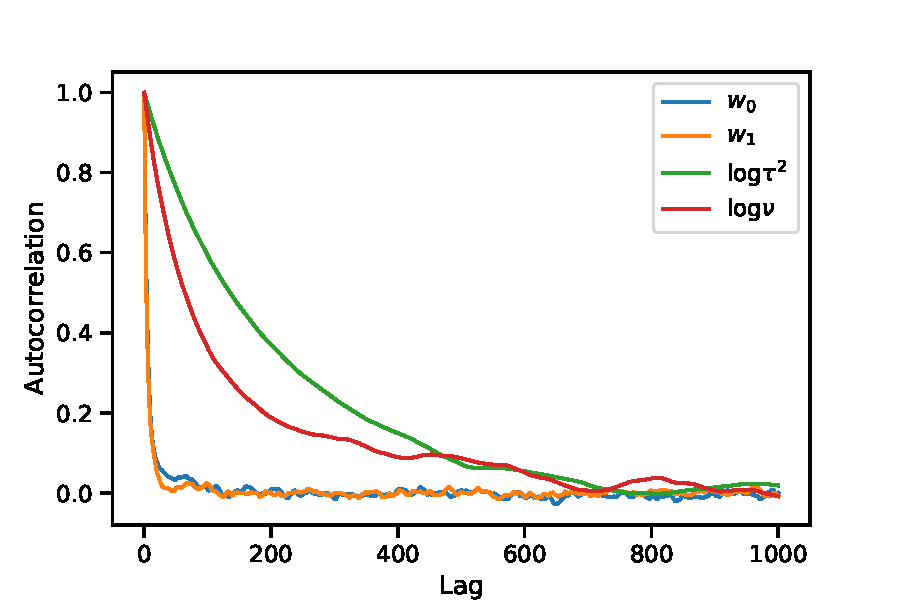
\includegraphics[width=0.6\textwidth]{figures/lap3/mh_autocorr.pdf}
    \end{center}
    Effective sample sizes (per 100,000 samples): 5629, 7235,  257, and 364.
\end{frame}

\begin{frame}{Autocorrelation of a Random Walk}
[From Geyer, 2011] To get some intuition, consider the following Markov chain,
\begin{align}
    \theta_s &= \rho \theta_{s-1} + \epsilon_s 
\end{align}
where $\epsilon_s \sim \cN(0, \tau^2)$.

MH isn't quite a mean-reverting random walk, but that's not a terrible model. 

In this toy example, we can calculate the autocovariance of the identity functional $f(\theta) = \theta$,
\begin{align}
    \mathrm{Cov}[\theta_s, \theta_{s+\ell}] = 
    \rho \mathrm{Cov}[\theta_s, \theta_{s+\ell - 1}] = 
    \rho^{\ell - 1} \mathrm{Cov}[\theta_s, \theta_{s+1}] = 
    \rho^\ell \Var[\theta_s]
\end{align}
so the autocorrelation function decays geometrically as $\mathrm{acf}(\ell) = \rho^\ell$.

At stationarity,
\begin{align}
    \Var[\theta_s] &= \Var[\theta_{s+1}] = \rho^2 \Var[\theta_s] + \tau^2
    \Rightarrow \Var[\theta_s] = \frac{\tau^2}{1 - \rho^2}
\end{align}

For $\rho^2 < 1$, the stationary distribution exists and is $\cN(0, \tfrac{\tau^2}{1-\rho^2})$.

\end{frame}

\begin{frame}{Autocorrelation of a Random Walk II}

Letting $f(\theta) = \theta$, we have,
\begin{align}
 \Var[\hat{f}] &= \frac{1}{S} \left( \Var[\theta] + 2 \sum_{\ell=1}^S \mathrm{Cov}[\theta_s, \theta_{s+\ell}] \right) \\
 &= \frac{1}{S} \cdot \Var[\theta] \left(1  + 2 \sum_{\ell=1}^S \rho^\ell \right) \\
 &\approx \frac{1}{S} \cdot \Var[\theta] \left(1  + 2 \frac{\rho}{1 - \rho} \right) & \text{(for large $S$)}\\
 &= \frac{1}{S} \cdot \Var[\theta] \cdot \frac{1 + \rho}{1 - \rho}
\end{align}
and 
\begin{align}
    S_{\mathsf{eff}} &= S \cdot \frac{1-\rho}{1+\rho}.
\end{align}
As $\rho \to 0$, we recover ordinary Monte Carlo. As $\rho \to 1$, the autocorrelation causes the variance of the estimator to blow up and the effective sample size to go to zero.

\end{frame}

\begin{frame}{What about bias?}

The mean squared error (MSE) of the estimator is determined by both the bias and the variance.

Ordinary Monte Carlo estimates are unbiased by construction, but MCMC estimates are only \textit{asymptotically unbiased}.

Bias is introduced whenever the initial distribution $\pi_1(\mbtheta)$ differs from the stationary distribution; i.e. in all practical cases!

Fortunately, the bias decays as $O(S^{-1})$ whereas the variance decays as $O(S^{-1/2})$, so asymptotically the MSE is dominated by the variance. 
    
\end{frame}



\section{Algorithm II: Hamiltonian Monte Carlo}
\label{sec:hmc}

\begin{frame}{Lap 3: Robust regress models and Intro to MCMC}
\begin{itemize}
    \item \hyperref[sec:robust_regression]{Model: Robust regression models}
    \item \hyperref[sec:intro_mcmc]{Algorithm: Intro to Markov chain Monte Carlo (MCMC)}
    \item \hyperref[sec:diagnostics]{Criticism: MCMC Diagnostics}
    \item \hyperref[sec:hmc]{\textbf{Algorithm II: Hamiltonian Monte Carlo}}
\end{itemize}
\end{frame}

\begin{frame}{How can we make smarter proposals?}
    Metropolis-Hastings with a symmetric Gaussian proposal behaves like a random walk.
    
    \citet{Neal2012-ev} argues that in $D$ dimensions, random walk MH needs $O(D^2)$ iterations to get an independent sample. 
    
    Can we develop more efficient transition distributions?
    
    Yes, if we have more information about the log probability. 
    
    For example, suppose that the log probability $\log p(\theta)$ is differentiable. We can use the gradient to make proposals that move farther and are more likely to be accepted.
\end{frame}

% Random walk behavior (back of the envelope calculations)?

% Metropolis Adjusted Langevin Algorithm (What if we have gradient information?)
\begin{frame}{Metropolis Adjusted Langevin Algorithm (MALA)}

The \textit{Metropolis-Adjusted Langevin Algorithm} uses the gradient of the log probability to make asymmetric proposals,
\begin{align}
    q(\mbtheta' \mid \mbtheta) &= \cN(\mbtheta + \tau \nabla_{\mbtheta} \log p(\mbtheta, \cD), \, 2\tau^2 \mbI) 
\end{align}
\textbf{Note:} $q(\mbtheta' \mid \mbtheta) \neq q(\mbtheta \mid \mbtheta')$! To calculate the acceptance probability, you need the gradient at both points.

MALA can be motivated as a discrete-time approximation to the \textit{Langevin} diffusion, a continuous-time stochastic differential equation for modeling molecular dynamics.

In high dimensions, the extra information provided by the gradient can lead to much more efficient chains. Neal argues that MALA needs $O(D^{4/3})$ computation to produce an independent sample.

But why stop at one gradient step?

\end{frame}

% Back of the envelope calculations O(d^{4/3})

% The three Hamilton's
\begin{frame}{Three Hamiltons}
\centering
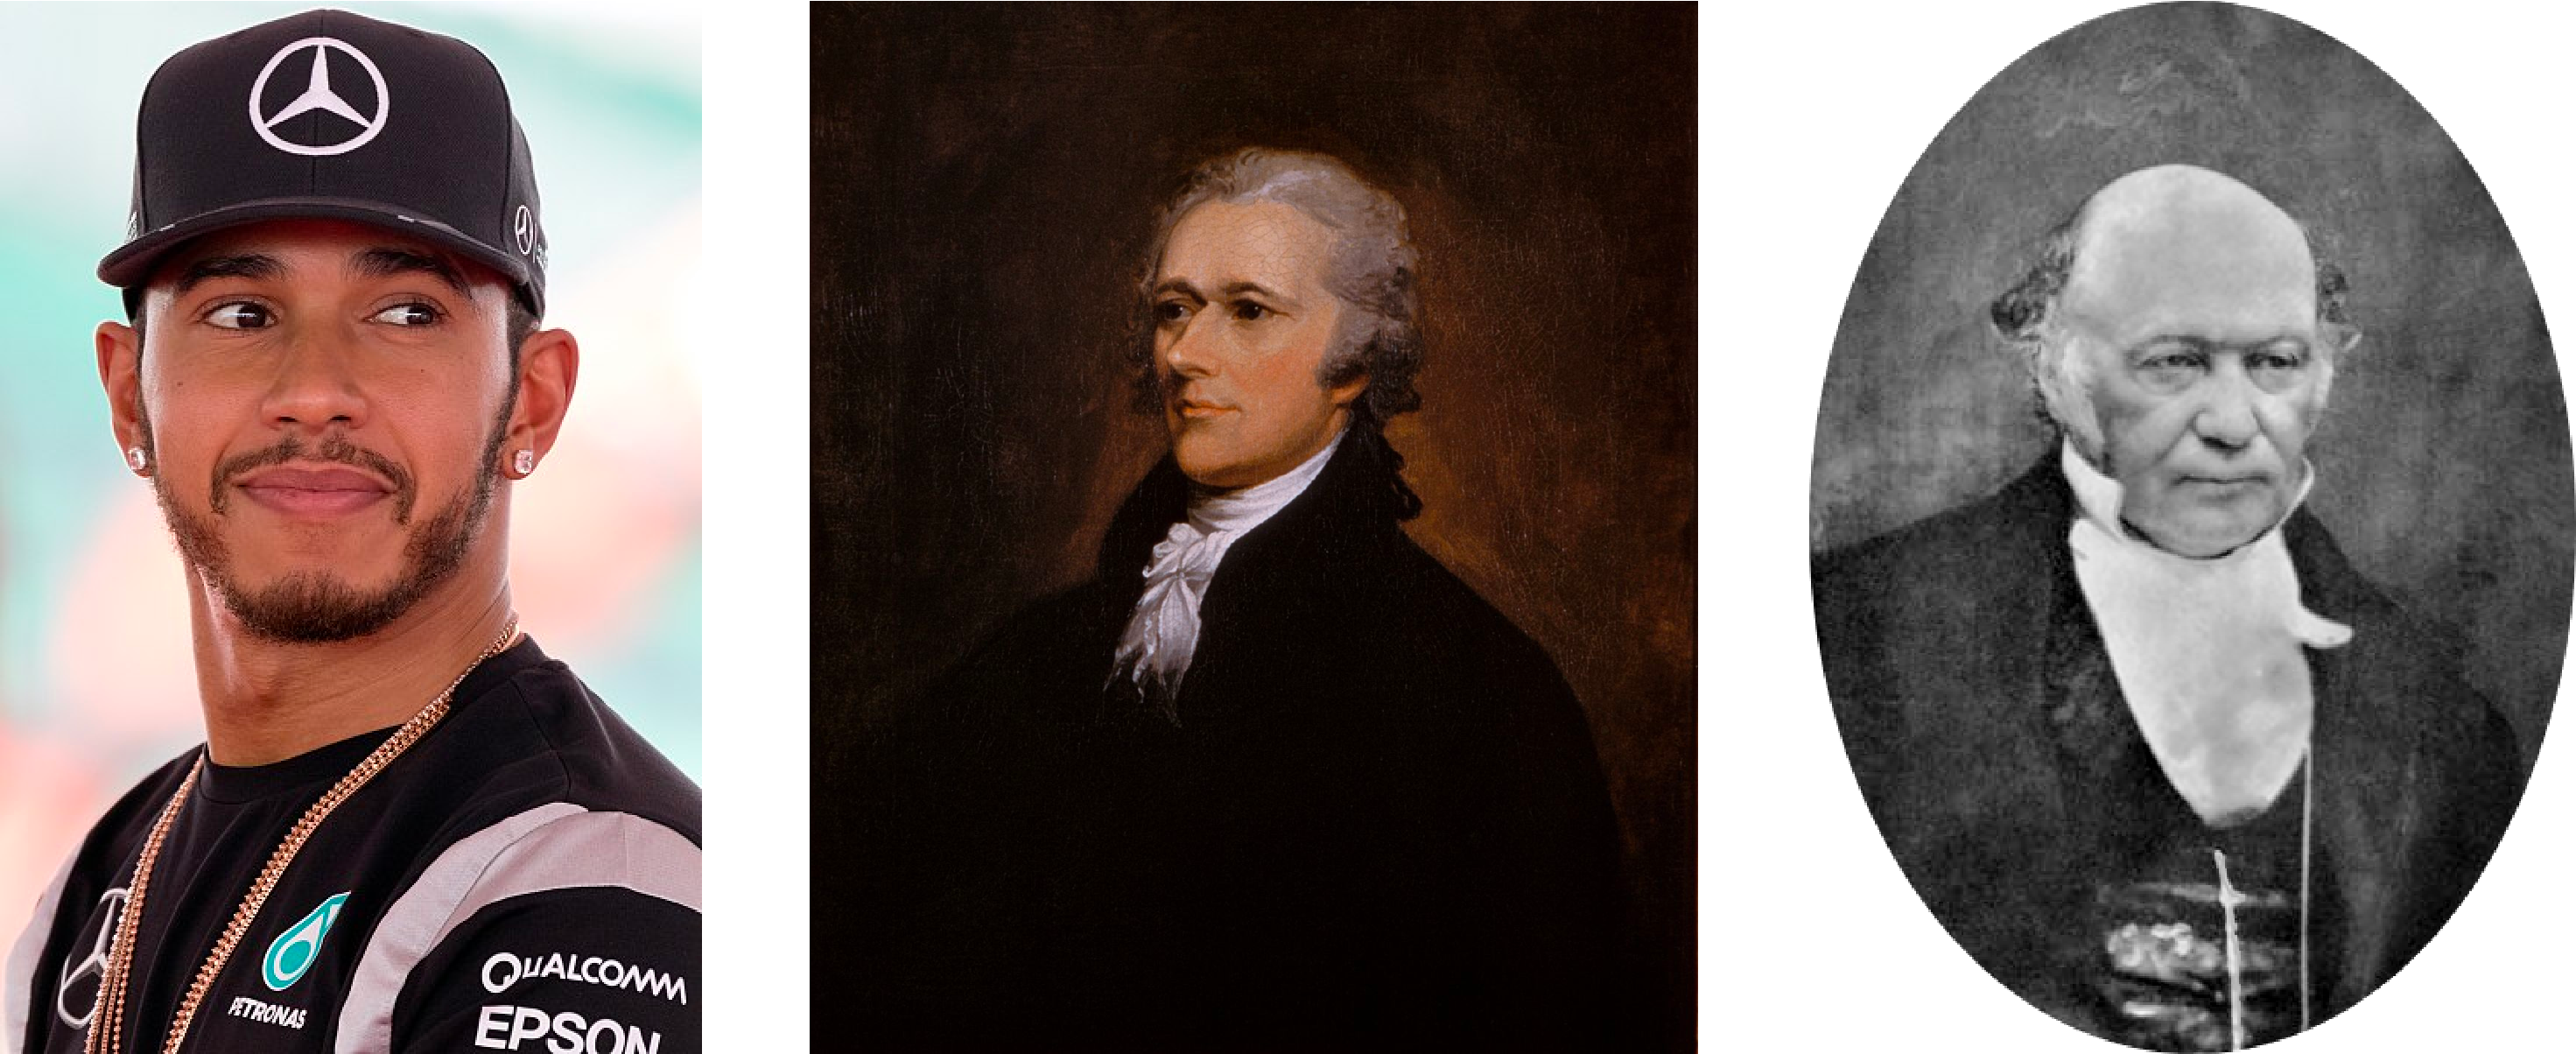
\includegraphics[width=0.95\textwidth]{figures/lap3/hamiltons.png}
\end{frame}

% Hamiltonian Monte Carlo intuition
% - first order information (gradients)
% - energy landscape
% - sliding puck
\begin{frame}{Hamiltonian Monte Carlo}
    
\textbf{Reference:} \citet{Neal2012-ev} \textit{{MCMC} using Hamiltonian dynamics}.

\textbf{Idea: } \textit{Think of negative log probability as an \textit{energy landscape}. Now imagine a puck sliding around on this bumpy surface. Give it random kicks; it will tend to slide downhill toward points of low potential energy (high probability). Each kick can displace the puck by a large amount. Done properly, the puck will visit points with probability proportional to the posterior probability. }
    
\end{frame}

\begin{frame}{Notation}
    
    Following \citet{Neal2012-ev}, let
    
    \begin{itemize}
        \item $\mbq \in \reals^D$ denote the \textit{position}; i.e. the current parameters (previously $\theta$)
        \item $\mbp \in \reals^D$ denote the \textit{momentum}; auxiliary variables that we don't care about, but which are necessary for HMC.
        \item $\mbz = [\mbq, \mbp]^\top \in \reals^{2D}$ denote the combined \textit{state of the system}.
        \item $\mbM$ denote the \textit{mass matrix}, another artificial construct. Typically, this will be $m \mbI$
        \item $U(\mbq)$ denote the \textit{potential energy}
        \item $K(\mbp) = \frac{1}{2} \mbp^\top \mbM^{-1} \mbp$ denote the \textit{kinetic energy}
    \end{itemize}
    
\end{frame}

% Hamilton's equations
\begin{frame}{Hamiltonian dynamics}
    The \textit{Hamiltonian} is the sum of the potential $H(\mbq, \mbp) = U(\mbq) + K(\mbp)$.
    
    The partial derivatives determine how the state evolves over time,
    \begin{align}
        \frac{\dif q_d}{\dif t} &= \frac{\partial H}{\partial p_d} = [\mbM^{-1} \mbp]_d \\
        \frac{\dif p_d}{\dif t} &= -\frac{\partial H}{\partial q_d} = -\frac{\partial  U}{\partial q_d}
    \end{align}
    for $d=1,\ldots, D$.
    
    Compactly,
    \begin{align}
        \frac{\dif \mbz}{\dif t} &= J \nabla H(z)
    \end{align}
    where 
    \begin{align}
        J &= \begin{bmatrix} \mbzero, \mbI \\ -\mbI, \mbzero
        \end{bmatrix}
    \end{align}
    
\end{frame}

\begin{frame}{One dimensional example}
    Consider the case where $D=1$ and $U(q) = \tfrac{1}{2}q^2$ and $K(p) = \tfrac{1}{2}p^2$.
    
    The partial derivatives are 
    \begin{align}
        \frac{\partial H}{\partial p} &= p \\
        -\frac{\partial H}{\partial q} &= -q
    \end{align}
    so 
    \begin{align}
        \frac{\dif \mbz}{\dif t} &= J \mbz.
    \end{align}
    
    This is a linear dynamical system, and the state at time $t+\Delta t$ is $\mbz(t+ \Delta t) = e^{J\Delta t} \mbz(t)$.
    
    Since $J \Delta t$ is skew-symmetric, the matrix exponential $e^{J \Delta t}$ is orthogonal. More precisely, $\mbz(t + \Delta t)$ is a rotation about the origin of $\mbz(t)$.
    
\end{frame}

\begin{frame}{Properties of Hamiltonian dynamics}

\begin{enumerate}
    \item \textbf{Reversibility: } The mapping from $z(t) \to z(t+ \Delta t)$ is one-to-one and invertible. To go from $z(t + \Delta t)$ to $z(t)$, negate $p(t + \Delta t)$, apply the the Hamiltonian dynamics for $\Delta t$ time, and negate the momentum again.
    
    \item \textbf{Conservation of energy: } The Hamiltonian (which is the total energy in a closed system) is conserved,
    \begin{align}
        \frac{\dif H}{\dif t} &= \sum_{d=1}^D \frac{\dif q_d}{\dif t} \frac{\partial H}{\partial q_d} + \frac{\dif p_d}{\dif t} \frac{\partial H}{\partial p_d} \\
        &= \sum_{d=1}^D \frac{\partial H}{\partial p_d} \frac{\partial H}{\partial q_d} - \frac{\partial H}{\dif q_d} \frac{\partial H}{\partial p_d} = 0.
    \end{align}
    
    
\end{enumerate}
    
\end{frame}

\begin{frame}[t]{Properties of Hamiltonian dynamics II}

\begin{enumerate}
    \item[3] \textbf{Volume preserving: } A set $R$ in $(q,p)$ space will have the same volume after being mapped through Hamiltonian dynamics. This follows from the fact that the divergence of the vector field is zero everywhere:
    \begin{align}
        \mathrm{div} \, \frac{\dif \mbz}{\dif t}
        = \sum_{d=1}^D \frac{\partial }{\partial q_d} \frac{\dif q_d}{\dif t} + \frac{\partial }{\partial p_d} \frac{\dif p_d}{\dif t}
        = \sum_{d=1}^D \frac{\partial }{\partial q_d} \frac{\partial H}{\partial p_d} - \frac{\partial }{\partial p_d} \frac{\partial H}{\partial q_d}
        = \sum_{d=1}^D \frac{\partial^2 H}{\partial q_d \partial p_d} - \frac{\partial^2 H}{\partial q_d \partial p_d} 
        = 0.
    \end{align}
    
    \item[4] \textbf{Sympleticness} Let $B$ be the Jacobian of the transformation from $\mbz(t) \to \mbz(t + \Delta t)$. It turns out that,
    \begin{align}
        B^\top J^{-1} B = J^{-1} 
    \end{align}
    which implies that $|B^\top| |J^{-1} | |B| = |J^{-1}|$ and thus $|B| = 1$. I.e. the dynamics preserve volume. 
\end{enumerate}
    
\end{frame}

\begin{frame}{Discretizing Hamilton's equations}

The properties above apply to the \textit{continuous time} Hamiltonian dynamics. Can we maintain them in practice?

\textbf{Idea: } In practice, to simulate $\Delta t$ elapsed time, we break it down into steps of size $\Delta t / \epsilon$.

\vspace{1em}

\begin{columns}
\begin{column}{.66\textwidth}
\textbf{Euler's method: } Update the state as,
\begin{align}
    \mbz(t+\epsilon) &= \mbz(t) + \epsilon \frac{\dif \mbz}{\dif t}\Big|_{\mbz(t)} \\
    \Rightarrow 
    p_d(t+\epsilon) &= p_d(t) - \epsilon \frac{\partial U}{\partial q_d} \Big|_{\mbq(t)} \\
    q_d(t+\epsilon) &= q_d(t) + \epsilon \frac{p_d(t)}{m_d}
\end{align}
Simple Euler integration does not preserve volume: trajectories eventually diverge, even with small $\epsilon$.
\end{column}

\begin{column}{.33\textwidth}
\centering
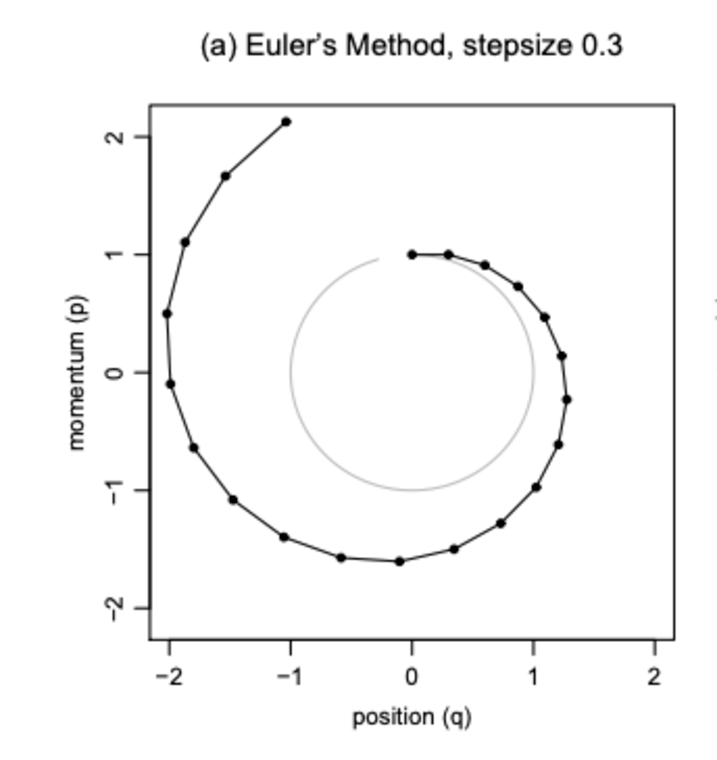
\includegraphics[width=\textwidth]{figures/lap3/euler.pdf}
\end{column}
\end{columns}

\end{frame}

\begin{frame}{The Leapfrog Integrator}

\begin{columns}
\begin{column}{.66\textwidth}
Instead, alternate updates of $p$ and $q$
\begin{align}
    p_d(t+\tfrac{\epsilon}{2}) &= p_d(t) - \frac{\epsilon}{2} \frac{\partial U}{\partial q_d} \Big|_{\mbq(t)} \\
    q_d(t+\epsilon) &= q_d(t) + \epsilon \frac{p_d(t+\tfrac{\epsion}{2})}{m_d} \\
    p_d(t+\epsilon) &= p_d(t + \tfrac{\epsilon}{2}) - \frac{\epsilon}{2} \frac{\partial U}{\partial q_d} \Big|_{\mbq(t + \epsilon)} \\
\end{align}
Each update is a \textit{shear transformation} in which only some variables change, by amounts that depend on the other, fixed variables. The determinant of such a transformation is one, so it preserves volume.
\end{column}

\begin{column}{.33\textwidth}
\centering
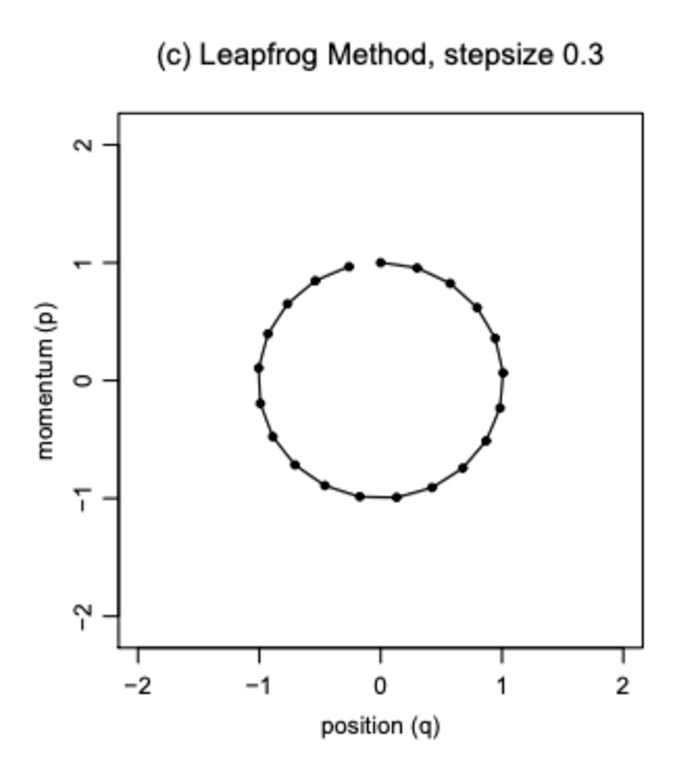
\includegraphics[width=\textwidth]{figures/lap3/leapfrog.pdf}
\end{column}
\end{columns}
    
\end{frame}

\begin{frame}{Using Hamiltonian dynamics for posterior inference}

Define a joint distribution on positions and momenta as,
\begin{align}
    p(\mbq, \mbp) &\propto \exp \left \{-H(\mbq, \mbp) \right \} \propto 
    \exp \left \{-U(\mbq) - K(\mbp)\right \}.
\end{align}

Now let $U(\mbq) = -\log p(\mbtheta = \mbq, \cD)$ be the \textit{negative} log joint probability. Then,
\begin{align}
    p(\mbq, \mbp) &= p(\mbtheta = \mbq \mid \cD) \times p(\mbp)
\end{align}
Samples of $\mbq$ will be marginally distributed according to the posterior $p(\mbtheta = \mbq \mid \cD)$.

Samples of $\mbp$ will be marginally distributed $p(\mbp) = \frac{\exp \{ -K(\mbp)\}}{\int_{\reals^D} \exp \{-K(\mbp)\} \dif \mbp}$. These are \textit{auxiliary variables} that we don't really care about---they're just there to help us construct MH proposals. 

We choose $K(\mbp)$ so $p(\mbp)$ is convenient; e.g. if $K(\mbp) = \frac{1}{2} \mbp^\top \mbM^{-1} \mbp$ then
\begin{align}
    p(\mbp) &= \cN(\mbp \mid \mbzero, \mbM).
\end{align}

\end{frame}

\begin{frame}{Hamiltonian Monte Carlo (HMC)}

\textbf{Hamiltonian Monte Carlo (HMC)} is Metropolis-Hastings on the joint distribution of $(\mbq, \mbp)$ with proposals based on Hamiltonian dynamics.

Starting at point $(\mbq', \mbp')$, sample the proposal distribution:
\begin{enumerate}
    \item Throw away $\mbp'$ and sample new momenta from their marginal distribution $\mbp \sim \cN(\mbzero, \mbM)$.
    \item Approximate Hamiltonian dynamics on $(\mbq, \mbp)$ for $\Delta t$ time using $L = \Delta t/\epsilon$ Leapfrog steps each of size $\epsilon$. Call the resulting point $(\mbq, \mbp)$.
    \item Flip the momentum $\mbp \leftarrow -\mbp$ to make the proposal symmetric.
\end{enumerate}

Then accept the proposed point $(\mbq, \mbp)$ with probability,
\begin{align}
    a((\mbq', \mbp') \to (\mbq, \mbp)) &= 
    \min \left\{1, \, \frac{\exp\{-H(\mbq, \mbp)\} \, q(\mbq', \mbp' \mid \mbq, \mbp)}{\exp\{-H(\mbq', \mbp')\} q(\mbq, \mbp \mid \mbq', \mbp')} \right \}
    =
    \min \left\{1, \, \frac{\exp\{-H(\mbq, \mbp)\}}{\exp \{-H(\mbq', \mbp')\}} \right \}.
\end{align}
If the Hamiltonian dynamics were simulated exactly, HMC would always accept. In practice, differences arise from numerical integration errors.

\end{frame}

\begin{frame}{HMC Dynamics on a Correlated 2D Gaussian}

\centering
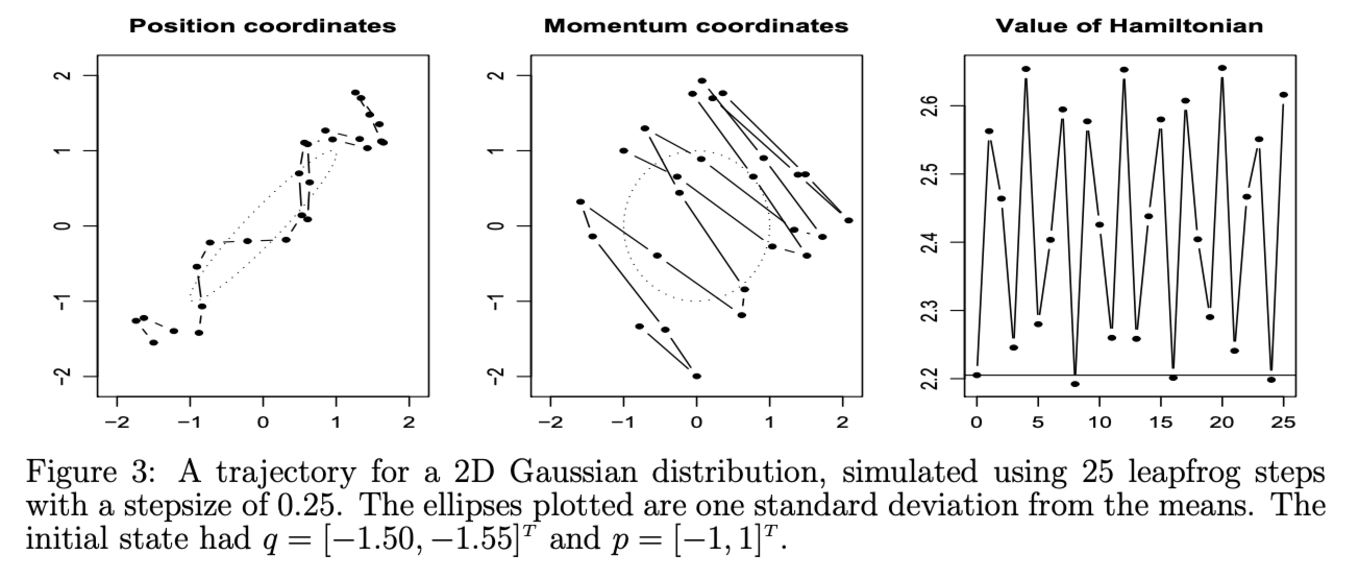
\includegraphics[width=0.9\textwidth]{figures/lap3/hmc_2d.pdf}
    
\end{frame}

\begin{frame}{HMC vs Random Walk MH}

\centering
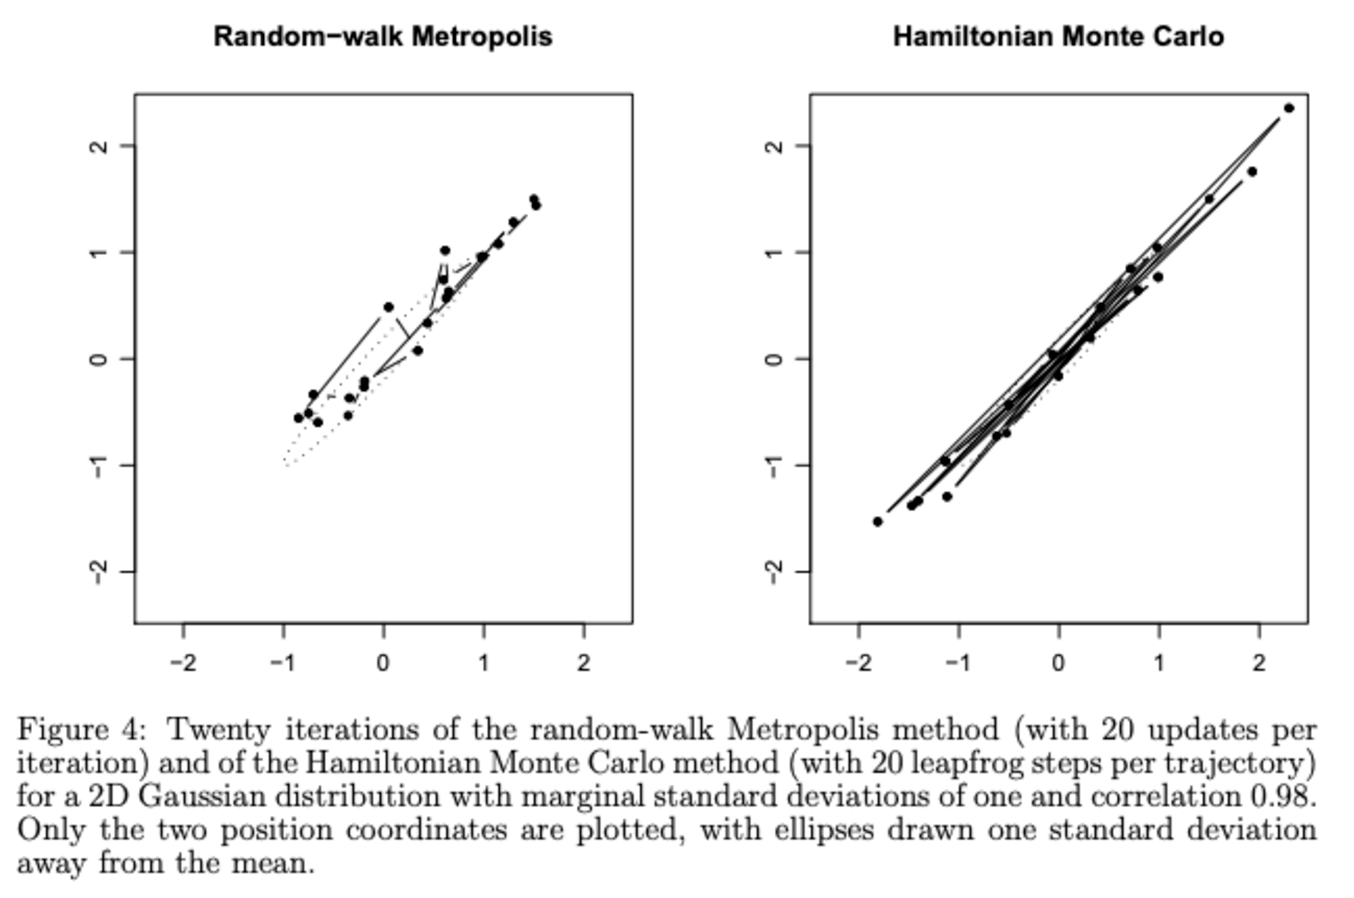
\includegraphics[width=0.8\textwidth]{figures/lap3/hmc_2d_comparison.pdf}
    
\end{frame}


\begin{frame}{HMC vs Random Walk MH II}
\centering
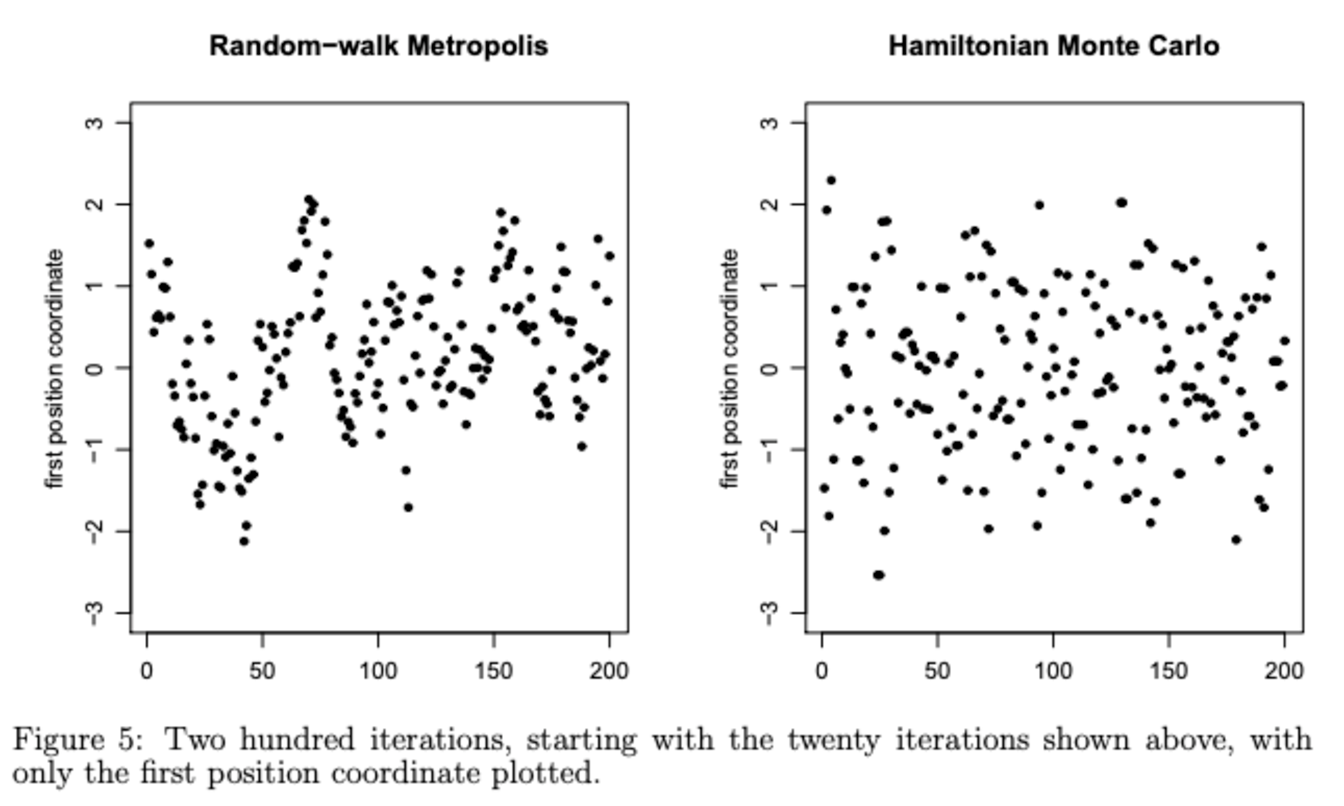
\includegraphics[width=0.8\textwidth]{figures/lap3/hmc_2d_traces.pdf}
\end{frame}

\begin{frame}{HMC vs Random Walk MH in 100D}
\centering
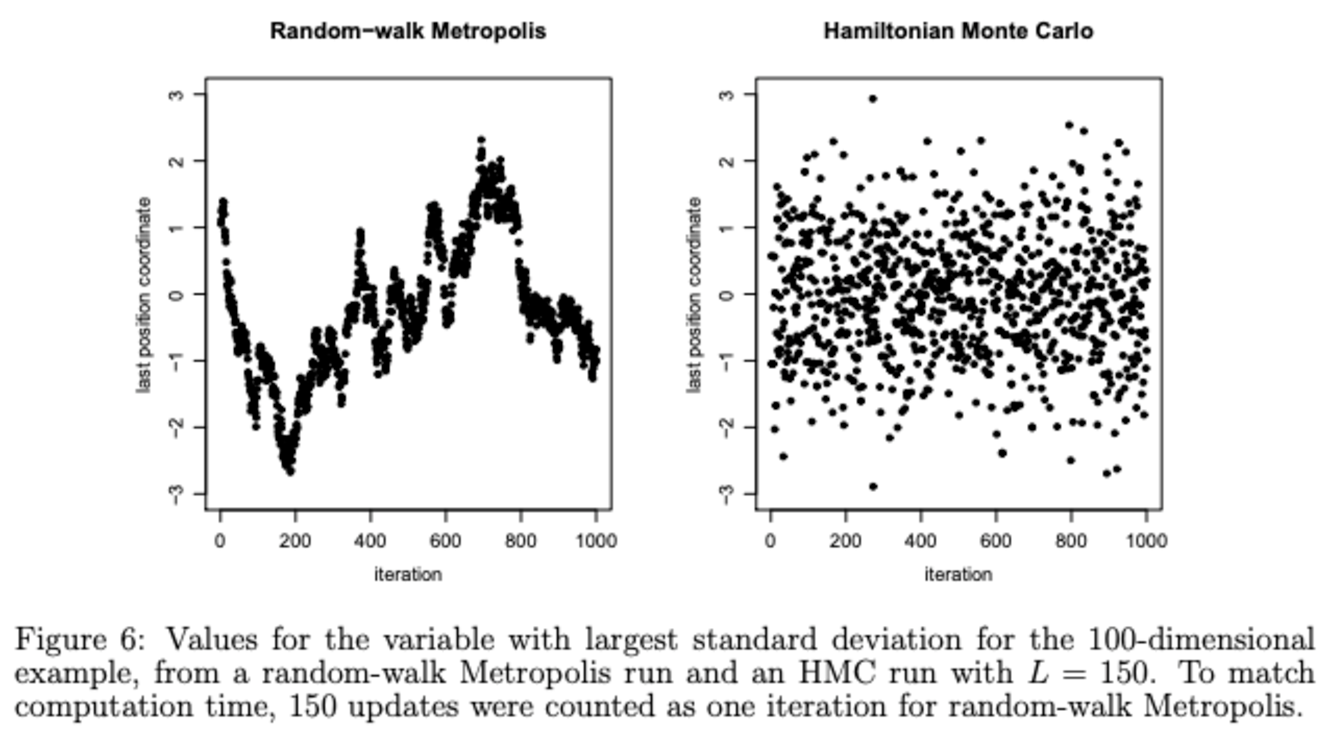
\includegraphics[width=0.8\textwidth]{figures/lap3/hmc_100d.pdf}
\end{frame}

\begin{frame}{HMC vs Random Walk MH in 100D II}
\centering
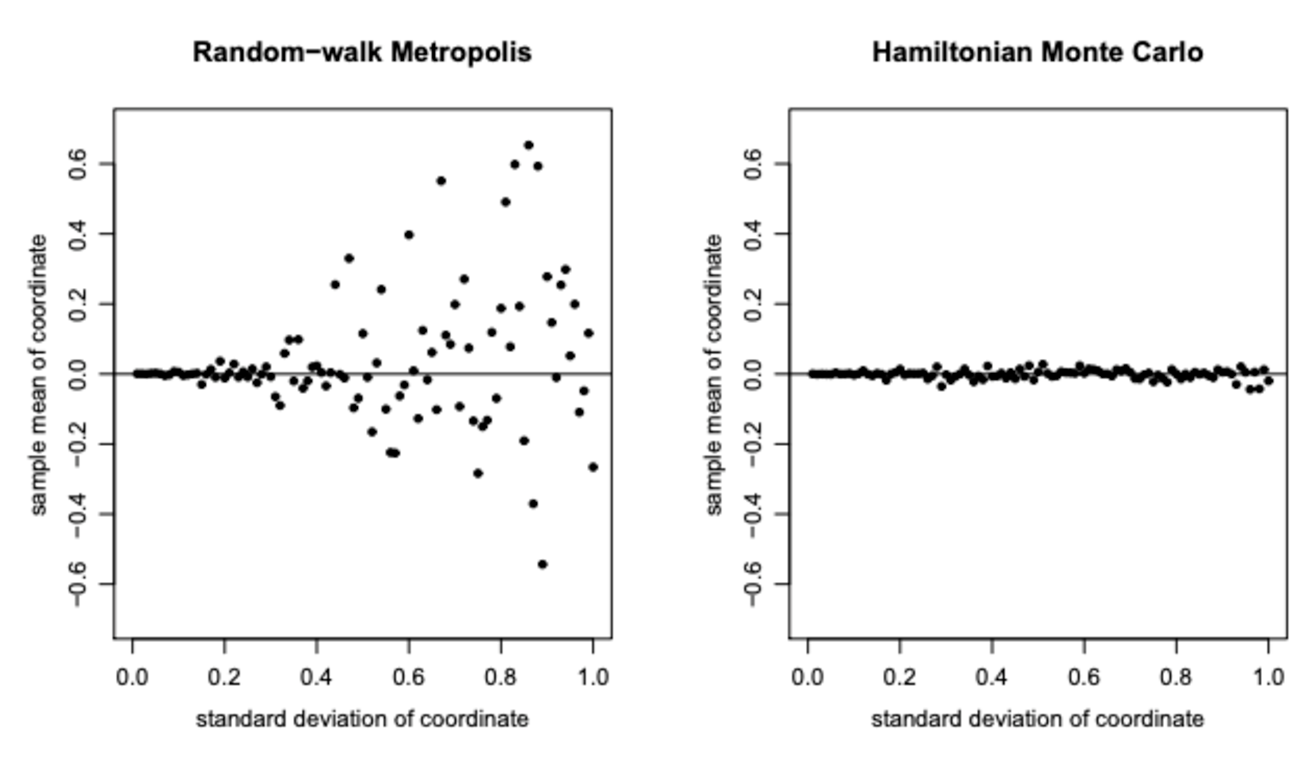
\includegraphics[width=0.8\textwidth]{figures/lap3/hmc_100d_mean.pdf}
\end{frame}

\begin{frame}{Benefits of avoiding random walks}
    
\begin{itemize}
    \item To maintain reasonably high acceptance probability, random walk MH needs proposal standard deviation (s.d.) comparable to the s.d. in the most constrained dimension (0.14 in the 2D Gaussian example and 0.01 in the 100D example).
    
    \item Num. iterations needed for RW-MH to reach an approximately independent state is proportional to the \emph{square} of the largest standard deviation to the smallest; i.e. to the condition number of the covariance matrix. 
    
    \item In contrast, integrating the Hamiltonian makes many steps in the same direction. The number of integration steps to reach an independent state is about the ratio of the largest s.d. to the smallest; i.e. the square root of the condition number.
    
    \item \citet{Neal2012-ev} argues that the number of leapfrog updates to reach an independent point scales as $O(D^{5/4})$, better than the $O(D^2)$ and $O(D^{4/3})$ estimates for random walk MH and MALA, respectively. 
    
    \item However, we still need to tune the step size $\epsilon$ to be comparable to the smallest s.d. 
    
\end{itemize}
    
\end{frame}

\begin{frame}{Adapting the step size}

\begin{itemize}
    \item A simple strategy is to tune the step size adaptively during the initial run of the Markov chain.

    \item For example, set a target acceptance rate (Neal argues that it should be around 0.65), then increase the step size if you're accepting too often and decrease if you're rejecting too often. 

    \item \citet{Andrieu2008-yc} proposed a widely-used multiplicative update scheme; it is the default in \href{https://www.tensorflow.org/probability/api_docs/python/tfp/mcmc/SimpleStepSizeAdaptation}{\texttt{tfp.mcmc.SimpleStepSizeAdaptation}}.
    
    \item The \textbf{No U-Turn Sampler (NUTS)} \citep{Hoffman2014-fl} adapts the distance traveled in response to the curvature of the target density. Conceptually, it continues until the trajectory turns back on itself (hence the name, ``No U-Turn'')
    
    \item More details can be found in \citet{Betancourt2017-ml}.
\end{itemize}

\end{frame}

\begin{frame}{Demos}
    
    \centering
    \url{https://chi-feng.github.io/mcmc-demo/app.html}
    
\end{frame}

\begin{frame}[t,allowframebreaks]
        \frametitle{References}
        \bibliographystyle{unsrtnat}
        \bibliography{refs.bib}
\end{frame}

\end{document}